% ====================================================================
% MAIN LaTeX FILE - SKRIPSI FASILKOM UNEJ
% ====================================================================
% STRUKTUR DOKUMENTASI SKRIPSI FASILKOM UNEJ - VERSI 2.0 (2023)
% Berdasarkan Juknis dan Keputusan Rektor UNEJ Nomor 5157/UN25/EP/2023
%
% ARSITEKTUR MODULAR & CLEAN:
% File ini adalah file utama (entry point) yang memanggil file-file
% terpisah untuk konfigurasi dan konten. Struktur ini memudahkan
% maintenance, kolaborasi, dan reusability.
%
% QUICK START:
% 1. Edit metadata.tex dengan informasi Anda
% 2. Compile: pdflatex main.tex (atau gunakan build tool)
% 3. Generated: main.pdf
%
% ====================================================================

% --- DOKUMEN CLASS & OPTIONS ---
% report = style untuk skripsi/thesis
% 12pt = ukuran font sesuai juknis
% a4paper = ukuran kertas A4
% oneside = single-sided printing
\documentclass[12pt, a4paper, oneside]{report}

% ====================================================================
% SECTION 1: LOAD METADATA & KONFIGURASI
% ====================================================================
% Metadata berisi semua variable/command yang dapat diubah
% (judul, nama penulis, pembimbing, dll.)

% ====================================================================
% METADATA DOKUMEN
% ====================================================================
% File ini berisi informasi umum tentang dokumen skripsi.
% EDIT BAGIAN INI SESUAI DENGAN DATA MAHASISWA DAN JUDUL SKRIPSI
% ====================================================================

% --- Informasi Penulis ---
\newcommand{\authorName}{Moh. Yusril Maqoshidana}
\newcommand{\studentID}{222410102064}
\newcommand{\studyProgram}{Program Studi Teknologi Informasi}
\newcommand{\faculty}{Fakultas Ilmu Komputer}
\newcommand{\university}{Universitas Jember}
\newcommand{\graduationYear}{2026}

% --- Judul Skripsi (sesuai format juknis: FRASA BUKAN KALIMAT) ---
\newcommand{\titleLine}{Sistem Analisis Topik Grup WhatsApp Berbasis Web Menggunakan BERTopic dengan IndoBERTweet dan BIRCH Clustering}
\newcommand{\titleUpperCase}{\MakeUppercase{Sistem Analisis Topik Grup WhatsApp Berbasis Web Menggunakan BERTopic dengan IndoBERTweet dan BIRCH Clustering}}

% --- Pembimbing dan Penguji ---
\newcommand{\supervisor}{Dr. Brian Rizqi Paradisiaca Darnoto, S.Kom., M.Kom}
\newcommand{\supervisorNIP}{199804272024061001}
\newcommand{\examinerOne}{Khoirunnisa' Afandi, S.Kom., M.Kom}
\newcommand{\firstExaminerNIP}{199412282024062001}
\newcommand{\examinerTwo}{Dony Bahtera Firmawan, S.Kom., M.Kom}
\newcommand{\secondExaminerNIP}{199711202024061001}

% --- Kata Kunci ---
\newcommand{\keywordOne}{Kata Kunci Satu}
\newcommand{\keywordTwo}{Kata Kunci Dua}
\newcommand{\keywordThree}{Kata Kunci Tiga}

% --- Tanggal Ujian ---
\newcommand{\examinationDate}{01 Juni 2026}


% ====================================================================
% SECTION 2: LOAD PACKAGES & KONFIGURASI GLOBAL
% ====================================================================
% Semua paket LaTeX diimport dari file terpisah untuk clarity

% Packages: encoding, bahasa, font, layout
% ====================================================================
% KONFIGURASI PAKET LaTeX
% ====================================================================
% File ini berisi semua paket (packages) yang digunakan dalam dokumen.
% Paket-paket diorganisir berdasarkan fungsi untuk kemudahan pemeliharaan.
%
% JANGAN MENAMBAHKAN \documentclass DI SINI - hanya \usepackage
% ====================================================================

% --- PAKET ENCODING & BAHASA ---
% Paket untuk encoding karakter UTF-8 dan dukungan bahasa Indonesia
\usepackage[utf8]{inputenc}                 % Encoding input UTF-8
\usepackage[T1]{fontenc}                    % Encoding font
\usepackage[indonesian]{babel}              % Dukungan bahasa Indonesia

% --- PAKET FONT & FORMATASI DASAR ---
% Mengatur jenis font dan margin sesuai juknis UNEJ
\usepackage{times}                          % Font Times New Roman (sesuai juknis)
\usepackage[top=4cm, left=4cm, bottom=3cm, right=3cm]{geometry}  % Margin sesuai juknis
\usepackage{setspace}                       % Pengaturan spasi antar baris
\usepackage{listings}

% --- PAKET KUSTOMISASI VISUAL STRUKTUR ---
% Paket untuk mengatur format judul bab, section, dan elemen visual lainnya
\usepackage{titlesec}                       % Kustomisasi judul chapter/section
\usepackage{fancyhdr}                       % Header dan footer custom
\usepackage{caption}                        % Pengaturan caption gambar/tabel

% --- PAKET KONTEN & REFERENSI ---
% Paket untuk menyisipkan berbagai elemen konten
\usepackage{graphicx}                       % Menyisipkan gambar (PNG, JPG, PDF)
\usepackage{booktabs}                       % Tabel berkualitas tinggi (profesi)
\usepackage{tabularx}                       % Tabel dengan kolom yang fleksibel
\usepackage{longtable}                      % Tabel multi-halaman
\usepackage{array}                          % Format kolom tabel lanjutan
\usepackage{float}                          % Opsi penempatan float seperti [H]
\usepackage{multirow}                       % Baris multi pada tabel
\usepackage{enumitem}                       % Kustomisasi list (mis. opsi [nosep])
\usepackage{amsmath}                        % Notasi matematika advanced
\usepackage{amssymb}                        % Simbol matematika tambahan
\usepackage{natbib}                         % Manajemen referensi (APA Style)
\usepackage{lipsum}                         % Teks dummy untuk placeholder (opsional)

% --- PAKET HYPERLINK & INTERAKTIF ---
% Paket untuk membuat dokumen PDF interaktif dengan hyperlink
\usepackage{hyperref}                       % Hyperlink dalam PDF
\usepackage{tocloft}                        % Kustomisasi daftar isi/tabel/gambar
\usepackage{afterpage}                       % Menunda perintah sampai halaman berikutnya (untuk page style)
\usepackage{indentfirst}                    % Indent paragraf pertama setelah heading
\usepackage{soul}                      % Highlighting teks (opsional, untuk revisi atau catatan)

% --- PAKET TAMBAHAN (OPSIONAL) ---
% Paket tambahan yang mungkin diperlukan:
\usepackage{subcaption}
% \usepackage{listings}                     % Untuk menampilkan kode sumber
% \usepackage{xcolor}                       % Dukungan warna tambahan
% \usepackage{tikz}                         % Menggambar diagram dan grafik
% \usepackage{array}                        % Pengaturan array dan tabel lebih lanjut
% \usepackage{multicol}                     % Multiple columns layout
% \usepackage{appendix}                     % Paket untuk lampiran (sudah built-in)

% ====================================================================
% PENGATURAN SPASI GLOBAL
% Sesuai juknis: 1.5 spasi untuk isi dokumen
% ====================================================================
\setstretch{1.5}  % Atur spasi antar baris menjadi 1.5


% Konfigurasi hyperref: metadata PDF, warna link, dll.
% ====================================================================
% KONFIGURASI HYPERREF
% ====================================================================
% File ini mengatur perilaku hyperlink dan PDF properties.
% Hyperlink dikonfigurasi untuk warna hitam (sesuai standar formal).
% ====================================================================

\hypersetup{
    colorlinks=true,
    linkcolor=black,
    citecolor=black,
    urlcolor=black
}


% Konfigurasi format chapter/section/subsection
% ====================================================================
% KONFIGURASI FORMAT STRUKTUR DOKUMEN
% ====================================================================
% File ini mengatur format untuk chapter, section, subsection, dll.
% Format disesuaikan dengan Juknis UNEJ Versi 2.0 (2023)
%
% Ketentuan:
% - Chapter (BAB): 14pt, Bold, All Caps, Centered
% - Section (bagian): Bold, Normal size, Penomoran
% - Subsection & Subsubsection: Bold, Normal size
% ====================================================================

% --- KONFIGURASI CHAPTER (BAB) ---
% Format: Centered, Bold, All Caps (14pt sesuai Juknis)
% Spasi sebelum: -20pt, sesudah: 40pt
\titleformat{\chapter}[block]
  {\bfseries\fontsize{14pt}{16pt}\selectfont\centering}
  {\MakeUppercase{\chaptertitlename} \thechapter.\hspace{0.5em}}
  {0pt}
  {\MakeUppercase}

\titlespacing*{\chapter}{0pt}{-20pt}{40pt}  % Spacing: normal, before=-20pt, after=40pt

% --- KONFIGURASI SECTION (Bagian 1) ---
% Format: Bold, Normal size (12pt), Bernomor
\titleformat{\section}
  {\bfseries\normalsize}               % Style: Bold, Normal size
  {\thesection}                        % Label: "1", "1.1", dll
  {0.5em}                                % Space antara label dan title
  {}                                   % Formatting title (none)

% --- KONFIGURASI SUBSECTION (Bagian 1.1) ---
% Format: Bold, Normal size (12pt), Bernomor
\titleformat{\subsection}
  {\bfseries\normalsize}               % Style: Bold, Normal size
  {\thesubsection}                     % Label: "1.1", "1.1.1", dll
  {0.5em}                                % Space antara label dan title
  {}                                   % Formatting title (none)

% --- KONFIGURASI SUBSUBSECTION (Bagian a., b., dll) ---
% Format: Normal font (12pt, tidak bold), Format huruf kecil (a., b., dll)
% Tidak masuk ke Daftar Isi (tocdepth = 2)
\setcounter{secnumdepth}{3}
\setcounter{tocdepth}{2}
\renewcommand{\thesubsubsection}{\alph{subsubsection}.}
\titleformat{\subsubsection}[block]
  {\normalfont\normalsize}             % Style: Normal font (TIDAK BOLD), Normal size
  {\hspace*{0.5cm}\thesubsubsection}   % Label: "a.", "b.", dll (menjorok sedang 0.5cm)
  {0.5em}                              % Space antara label dan title
  {}                                   % Formatting title (none)

\titlespacing*{\subsubsection}{0pt}{10pt}{4pt}  % Spacing: indent=0pt, before=10pt, after=4pt

% --- KONFIGURASI PARAGRAPH ---
% Untuk case yang lebih spesifik (jarang digunakan dalam juknis)
\titleformat{\paragraph}[runin]
  {\bfseries}
  {\theparagraph}
  {0.5em}
  {}

% --- KONFIGURASI IDENTASI ---
\setlength{\parindent}{1cm}  % Atur jarak indentasi

% --- KONFIGURASI KETEBALAN GARIS TABEL (STANDAR JURNAL AKADEMIK) ---
% Menyeragamkan ketebalan garis pada seluruh tabel (booktabs dan standard) agar rapi, proporsional, dan elegan
\setlength{\heavyrulewidth}{0.75pt}  % Garis atas (\toprule) & garis bawah (\bottomrule)
\setlength{\lightrulewidth}{0.45pt}  % Garis pemisah header (\midrule)
\setlength{\cmidrulewidth}{0.35pt}   % Garis sub-kolom (\cmidrule)
\setlength{\arrayrulewidth}{0.45pt}  % Garis pemisah standar (\hline pada tabular/longtable)
\setlength{\aboverulesep}{0.35ex}    % Jarak vertikal di atas garis booktabs
\setlength{\belowrulesep}{0.35ex}    % Jarak vertikal di bawah garis booktabs

% --- KONFIGURASI DAFTAR ISI / TABEL / GAMBAR ---
% Dipusatkan di file ini supaya styling tetap konsisten dengan struktur dokumen
\renewcommand{\cftchapleader}{\cftdotfill{\cftdotsep}}

% --- KONFIGURASI JUDUL DAFTAR ISI / TABEL / GAMBAR ---
% Menyamakan format judul dengan \chapter: Bold, 14pt, Centered, ALL CAPS

\renewcommand{\cfttoctitlefont}{%
  \hfill\bfseries\fontsize{14pt}{16pt}\selectfont\MakeUppercase
}
\renewcommand{\cftaftertoctitle}{\hfill}

\renewcommand{\cftlottitlefont}{%
  \hfill\bfseries\fontsize{14pt}{16pt}\selectfont\MakeUppercase
}
\renewcommand{\cftafterlottitle}{\hfill}

\renewcommand{\cftloftitlefont}{%
  \hfill\bfseries\fontsize{14pt}{16pt}\selectfont\MakeUppercase
}
\renewcommand{\cftafterloftitle}{\hfill}



% Hapus after-title skip default tocloft agar konsisten
\setlength{\cftaftertoctitleskip}{40pt}
\setlength{\cftafterlottitleskip}{40pt}
\setlength{\cftafterloftitleskip}{40pt}
\setlength{\cftbeforetoctitleskip}{-20pt}
\setlength{\cftbeforelottitleskip}{-20pt}
\setlength{\cftbeforeloftitleskip}{-20pt}


% Konfigurasi header/footer dan penomoran halaman
% ====================================================================
% KONFIGURASI HEADER, FOOTER, DAN PENOMORAN HALAMAN
% ====================================================================
% File ini mengatur penomoran halaman dan header/footer dokumen.
%
% Ketentuan Penomoran Juknis UNEJ:
% - Bagian Awal (Front Matter): Roman kecil (i, ii, iii, ...) di tengah bawah
% - Bagian Inti (Main Body): Angka Arab (1, 2, 3, ...) di kanan atas
% - Halaman pertama setiap BAB: Angka di tengah bawah (tanpa header)
% ====================================================================

% === STYLE UNTUK HALAMAN REGULER ===
% Nomor halaman di kanan atas, tanpa garis header
\fancypagestyle{plain}{%
	\fancyhf{}%
	\fancyfoot[C]{\thepage}%
	\renewcommand{\headrulewidth}{0pt}%
	\renewcommand{\footrulewidth}{0pt}%
}

% Style untuk halaman biasa bagian utama: nomor di kanan atas
\fancypagestyle{fancy}{%
	\fancyhf{}%
	\fancyhead[R]{\thepage}%
	\renewcommand{\headrulewidth}{0pt}%
	\renewcommand{\footrulewidth}{0pt}%
}





% ====================================================================
% CATATAN IMPLEMENTASI DI main.tex:
% 1. Bagian Front Matter harus menggunakan:
%    \pagenumbering{roman}
%    \pagestyle{plain}
%    Untuk penomoran Romawi (i, ii, iii) di tengah bawah
%
% 2. Bagian Main Body harus menggunakan:
%    \pagenumbering{arabic}
%    \setcounter{page}{1}
%    \pagestyle{fancy}
%    Untuk penomoran Arab (1, 2, 3) di kanan atas
% ====================================================================


% Custom commands & environments untuk DRY principle
% ====================================================================
% CUSTOM COMMANDS & ENVIRONMENTS
% ====================================================================
% File ini berisi custom command dan environment untuk mempermudah
% penulisan dan membuat dokumen lebih konsisten dan DRY (Don't Repeat Yourself).
%
% Tambahkan custom command di sini untuk:
% - Pengurangan kode yang berulang
% - Konsistensi formatting
% - Kemudahan modifikasi global
% ====================================================================

% --- COMMAND UNTUK CHAPTER TANPA NOMOR (Front Matter) ---
% Penggunaan lebih mudah daripada menulis \chapter* setiap kali
% Contoh: \frontmatterchapter{PERSEMBAHAN}
\newcommand{\frontmatterchapter}[1]{
  \chapter*{#1}
  \addcontentsline{toc}{chapter}{#1}
}

% --- COMMAND UNTUK KEYWORDS/KATA KUNCI ---
% Untuk konsistensi formatting kata kunci di abstrak
% Contoh: \keywords{Kata Kunci Satu, Kata Kunci Dua, Kata Kunci Tiga}
\newcommand{\keywords}[1]{
  \vspace{1cm}
  \noindent \textbf{Kata Kunci:} \textit{#1}
}

% --- COMMAND UNTUK KEYWORDS DALAM BAHASA INGGRIS ---
% Contoh: \keywordsen{Keyword One, Keyword Two, Keyword Three}
\newcommand{\keywordsen}[1]{
  \vspace{1cm}
  \noindent \textbf{Keywords:} \textit{#1}
}

% --- ENVIRONMENT UNTUK CENTERLINE (SHORTCUT) ---
% Penggunaan lebih singkat dari \begin{center} ... \end{center}
% Contoh: \mycenterline{\textit{``quoted text''}}
\newcommand{\mycenterline}[1]{
  \begin{center}
    #1
  \end{center}
}

% --- COMMAND UNTUK AUTHOR DENGAN AFFILIATION ---
% Berguna jika diperlukan dalam cover atau halaman judul
% Contoh: \authorWithAffiliation{Nama Mahasiswa}{NIM}{Program Studi}
\newcommand{\authorWithAffiliation}[3]{
  {\normalsize\bfseries #1}\\
  {\normalsize #2}\\
  {\normalsize #3}
}

% --- COMMAND UNTUK QUOTE YANG DIPUSATKAN ---
% Untuk mengformat quote atau motto dengan mudah
% Contoh: \quoteline{``In life, you either win or learn...''}{Nelson Mandela}
\newcommand{\quoteline}[2]{
  \begin{center}
    \textit{#1}\\[0.5cm]
    (\small\textit{#2})
  \end{center}
}

% --- COMMAND UNTUK HORIZONTAL RULE DEKORATIF ---
% Untuk separator visual dalam dokumen
\newcommand{\decorativeHRule}{
  \vspace{0.5cm}
  \centerline{\hrulefill}
  \vspace{0.5cm}
}

% --- COMMAND UNTUK TEMPAT TANDA TANGAN (SIGNATURE BLOCK) ---
% Berguna untuk halaman persetujuan
% Usage: \signatureBlock{Nama}{Tanggal}{Jabatan}
\newcommand{\signatureBlock}[3]{
  \vspace{1.5cm}
  \noindent
  #2\\
  \vspace{3cm}
  \noindent\line(1,0){100}\\
  \noindent\small #1\\
  \noindent\small #3
}

% --- COMMAND UNTUK INFORMASI PENELITIAN ---
% Shortcut untuk menampilkan info pembimbing, penguji, dll
% Contoh: \advisorInfo{Nama Pembimbing}{Gelar}
\newcommand{\advisorInfo}[2]{
  \noindent\textbf{#1}\\
  {\normalsize #2}
}

% --- COMMAND UNTUK BARIS NAMA & NIP PENGUJI/PEMBIMBING ---
\newcommand{\supervisorrow}[4]{%
  % #1 = nomor
  % #2 = jabatan (Pembimbing Utama / Penguji Utama / dst)
  % #3 = nama
  % #4 = NIP
  
  \quad #1. #2 & \\[0.3em]
  
  \quad \quad Nama : #3 & \signatureLine \\[0.3em]
  \quad \quad NIP \; : #4 & \\[1em]
}

% --- ENVIRONMENT TABEL PEMBIMBING & PENGUJI ---
\newenvironment{approvalboard}{%
  \noindent
  \begin{tabular}{@{} p{0.7\textwidth} p{0.3\textwidth} @{}}
}{%
  \end{tabular}
}

% --- GARIS TANDA TANGAN ---
\newcommand{\signatureLine}{(\dotfill)}

% --- COMMAND UNTUK SUBSUBSECTION KHUSUS (a., b., dll. - Normal font, Menjorok Lurus Angka Akhir Subsection) ---
% Penggunaan: \subsubsubsection{Judul Subsubsection}
\newcommand{\subsubsubsection}[1]{%
  \par\vspace{10pt}%
  \refstepcounter{subsubsection}%
  \hspace*{1.2cm}{\normalfont\normalsize \alph{subsubsection}. #1}\par\nopagebreak\vspace{4pt}%
}

% ====================================================================
% CATATAN PENGGUNAAN:
% - Gunakan custom command ini secara konsisten di seluruh dokumen
% - Jika perlu mengubah format, hanya perlu edit di sini (DRY principle)
% - Tambahkan command baru sesuai kebutuhan dokumen Anda
% ====================================================================


% ====================================================================
% SECTION 3: BEGIN DOCUMENT
% ====================================================================

\begin{document}

% ====================================================================
% BAGIAN 0: HALAMAN SAMPUL
% ====================================================================
% Halaman sampul adalah halaman pertama (tidak dinomori)

% ====================================================================
% HALAMAN SAMPUL
% ====================================================================
% File ini berisi halaman sampul skripsi sesuai Juknis UNEJ.
% Dokumentasi nama variabel ada di metadata.tex
% ====================================================================

\begin{titlepage}
	% Uncoment jika ingin melihat layout halaman
	% \layout
	\centering

	% Logo
	
\includegraphics[width=4cm]{images/logo.png}\par
	\vspace{1cm}

	% Judul
	{\bfseries
		\titleUpperCase\par}
	\vspace{1cm}

	\textit{Diajukan guna memenuhi salah satu syarat memperoleh gelar Sarjana pada \studyProgram}
	\vspace{1cm}

	{\bfseries \MakeUppercase{Skripsi} \par}
	\vfill

	% Nama
	{\bfseries Oleh: \par}
	{\bfseries \authorName \\
	NIM \studentID}

	\vfill

	% Identitas Program Studi
	{\bfseries \MakeUppercase{KEMENTERIAN PENDIDIKAN, KEBUDAYAAN, RISET, DAN TEKNOLOGI}
	\MakeUppercase{\studyProgram} \\
		\MakeUppercase{\faculty} \\
		\MakeUppercase{\university} \\
		\graduationYear}

\end{titlepage}


% ====================================================================
% BAGIAN 1: FRONT MATTER (BAGIAN AWAL)
% ====================================================================
% Penomoran: Angka Romawi kecil (i, ii, iii, ...) di tengah bawah

\pagenumbering{roman}
\pagestyle{plain}

% Halaman Persembahan (Dedication)
% ====================================================================
% HALAMAN PERSEMBAHAN
% ====================================================================
% File ini berisi halaman persembahan (dedikasi).
% EDIT konten sesuai keinginan Anda.
% ====================================================================

\frontmatterchapter{PERSEMBAHAN}

% --- ISI PERSEMBAHAN ---
% Ganti konten lipsum berikut dengan teks persembahan Anda
\noindent Halaman ini saya persembahkan kepada:

\begin{enumerate}[nosep]
    \item Allah SWT, atas segala rahmat, karunia, serta kemudahan yang diberikan sehingga penulis dapat menyelesaikan skripsi ini dengan baik.

    \item Bapak Subono dan Ibu Marsidah yang selalu mendoakan yang terbaik, mendukung segala usaha, serta selalu sabar dan percaya hingga sampai penulis mampu menyelesaikan pendidikan.

    \item Bapak \supervisor\ selaku Dosen Pembimbing Utama yang telah meluangkan waktu, memberikan arahan, bimbingan, serta masukan yang berharga selama proses penyusunan skripsi ini.

    \item Ibu \examinerOne dan Bapak \examinerTwo selalu dosen penguji yang memberikan saran dan masukan dalam proses pengembangan skripsi.

    \item Dosen Fakultas Ilmu Komputer, Universitas Jember yang telah memberikan ilmu dan pengalaman yang berharga selama masa perkuliahan.

    \item Sahabat yang telah memberikan dukungan, semangat, serta bantuan selama proses penyusunan skripsi ini.

\end{enumerate}

% Alternatif: Jika ingin format yang lebih singkat/padat, gunakan \lipsum:
% \lipsum[1-2]  % Ganti dengan paragraf Anda sendiri

\newpage


% Halaman Motto
% ====================================================================
% HALAMAN MOTTO
% ====================================================================
% File ini berisi halaman motto/semboyan.
% EDIT motto sesuai dengan pilihan Anda.
% ====================================================================

\frontmatterchapter{MOTTO}

\begin{center}
    
    % Motto Pertama (Barat/Sekuler)
    \textit{``In life, you either win or learn. When you lose, experience is the reward''} \\
    (Nelson Mandela) \\
    
    % Spasi antar motto
    \vspace{1cm}
    
    % Motto Kedua (Agama/Spiritual)
    \textit{``Dan orang-orang yang berjihad untuk (mencari keridhaan) Kami, benar-benar akan
    Kami tunjukkan kepada mereka jalan-jalan Kami''} \\
    (Al-Ankabut: 69)
    
    % Spasi di bawah motto
    \vspace{1cm}
    
    % Motto Ketiga (Opsional)
    % Uncomment baris berikut jika ingin menambahkan motto ketiga:
    % \textit{``Investasi terbaik adalah investasi pada diri sendiri''} \\
    % (Unknown)
\end{center}

\newpage

% ====================================================================
% CATATAN:
% - Maksimal 3 motto disarankan untuk keseimbangan visual
% - Pilih motto yang bermakna dan menginspirasi
% - Format: italic text dalam tanda petik + atribusi (penulis/sumber)
% ====================================================================


% Halaman Pernyataan Orisinalitas
% ====================================================================
% HALAMAN PERNYATAAN ORISINALITAS
% ====================================================================
% File ini berisi pernyataan keaslian/orisinalitas karya.
% Halaman ini harus bermaterai Rp10.000 (sesuai Juknis).
% EDIT nama penulis dan tanggal sesuai kebutuhan.
% ====================================================================

\frontmatterchapter{PERNYATAAN ORISINALITAS}

% --- PERNYATAAN FORMAL ---
\noindent Saya yang bertanda tangan di bawah ini:
\begin{itemize}[label={}, nosep]
    \item Nama: \authorName
    \item NIM: \studentID
\end{itemize}

\noindent Dengan ini menyatakan bahwa skripsi yang berjudul: \textit{``\titleUpperCase''} 

\noindent adalah benar-benar hasil karya saya sendiri. Saya juga menyatakan bahwa dalam skripsi ini tidak terdapat karya yang pernah diajukan untuk memperoleh gelar sarjana atau gelar lainnya di mana pun.

\noindent Saya bertanggung jawab atas kebenaran dan keorisinalan isi skripsi ini. Apabila dikemudian hari terbukti bahwa skripsi ini mengandung unsur plagiasi, maka saya siap menanggung akibat hukum yang berlaku.

% --- TEMPAT DAN TANGGAL PENANDATANGANAN ---
% \vspace{2cm}

Jember, \examinationDate

% --- TEMPAT MATERAI DAN TANDATANGAN ---
\vspace{1cm}

\noindent
\textbf{*Bermaterai Rp10.000}

\vspace{2cm}

\noindent\line(1,0){250}

\noindent\authorName

\noindent\studentID

\newpage

% ====================================================================
% CATATAN PENTING:
% 1. Halaman ini HARUS bermaterai Rp10.000 sebelum pengumpulan ke kampus
% 2. Tandatangan harus asli (tinta biru), bukan scan
% 3. Edit placeholder berikut di metadata.tex:
%    - \authorName
%    - \studentID
%    - \titleLine, \titleUpperCase
%    - \examinationDate
% ====================================================================


% Halaman Persetujuan & Pengesahan (Approval & Sign-off)
% ====================================================================
% HALAMAN PERSETUJUAN
% ====================================================================
% File ini berisi halaman persetujuan dari pembimbing dan penguji.
% Tanda tangan harus asli (tinta biru), bukan scan.
% EDIT nama-nama pembimbing dan penguji sesuai kebutuhan.
% ====================================================================

\frontmatterchapter{HALAMAN PERSETUJUAN}

\noindent Skripsi berjudul \textit{``\titleUpperCase''} telah diuji dan disetujui oleh \faculty\  \university\ pada:
  \begin{itemize}[leftmargin=0pt, labelsep=0pt, label={}]
    \item Hari: Minggu
    \item Tanggal: \examinationDate
    \item Tempat: \faculty \university
  \end{itemize}


% --- PEMBIMBING AKADEMIK ---
\vspace{2em}
\noindent
\begin{approvalboard}

Pembimbing & \multicolumn{1}{c}{Tanda Tangan} \\[0.5em]

\supervisorrow
{1}
{Pembimbing Utama}
{Dr. Brian Rizqi P. D., S.Kom., M.Kom}
{\supervisorNIP}

Penguji & \\[0.5em]

\supervisorrow
{1}
{Penguji Utama}
{\examinerOne}
{\firstExaminerNIP}

\supervisorrow
{2}
{Penguji Anggota 1}
{\examinerTwo}
{\secondExaminerNIP}

\end{approvalboard}

\newpage

% ====================================================================
% CATATAN PENTING:
% 1. Tanda tangan HARUS asli dengan tinta biru
% 2. Edit nama-nama di metadata.tex:
%    - \advisorOne
%    - \advisorTwo
%    - \examinerOne
%    - \examinerTwo
%    - \examinationDate
% 3. Tempat dapat diubah menjadi nama ruangan/gedung sesuai tempat ujian
% ====================================================================


% Abstrak Bahasa Indonesia
% ====================================================================
% ABSTRAK (BAHASA INDONESIA)
% ====================================================================
% File ini berisi abstrak dalam bahasa Indonesia (200-300 kata).
% EDIT konten sesuai dengan penelitian Anda.
% ====================================================================

\frontmatterchapter{ABSTRAK}

% --- ISI ABSTRAK ---
\noindent Tingginya aktivitas pertukaran pesan pada grup WhatsApp kerap memicu fenomena \textit{information overload}, yang menyulitkan pengguna dalam mengikuti dinamika diskusi dan menyaring informasi penting tanpa membaca riwayat pesan secara manual. Kendati teknik \textit{topic modeling} dapat mengekstraksi topik secara otomatis, penerapannya pada percakapan WhatsApp menghadapi tantangan teks pendek, struktur informal, derau tinggi, dan \textit{code-mixing}. Di samping itu, algoritma pengklasteran HDBSCAN pada \textit{framework} BERTopic standar mengeliminasi hingga 41\%--43\% data sebagai \textit{outlier}, sehingga menghilangkan banyak substansi percakapan penting.

Penelitian ini bertujuan mengembangkan modifikasi arsitektur BERTopic yang memadukan model \textit{embedding} IndoBERTweet, algoritma pengklasteran hierarkis BIRCH untuk menekan proporsi \textit{outlier}, serta skema pembobotan BM25 untuk representasi kata kunci topik. Model dievaluasi terhadap \textit{baseline} BERTopic menggunakan metrik \textit{Topic Coherence} (C-NPMI), \textit{Topic Diversity}, \textit{Embedding Density}, dan \textit{Intra-topic Similarity}, serta diimplementasikan ke dalam aplikasi analisis berbasis web.

Metodologi penelitian menerapkan pendekatan eksperimental dan R\&D menggunakan dataset 91.868 pesan grup WhatsApp Komunitas Buku (2023--2026) yang menghasilkan 56.089 dokumen bersih setelah \textit{Single-Path Preprocessing}. Pemodelan topik memadukan IndoBERTweet (768 dimensi), reduksi UMAP (5 dimensi), pengklasteran BIRCH, ekstraksi kata kunci BM25 dengan penyaringan \textit{stopwords} 9 kategori, serta reduksi topik otomatis. Sistem dibangun dengan arsitektur \textit{client-server} (Vue.js dan FastAPI) yang dilengkapi pemantauan progres \textit{real-time} berbasis SSE, penelusuran konteks pesan (\textit{traceability}), dan privasi data di sisi klien.

% --- KESIMPULAN (Belum diisi sesuai instruksi) ---
% Kesimpulan dan temuan empiris final akan dilengkapi setelah evaluasi menyeluruh.

\vspace{0.3cm}

% --- KATA KUNCI ---
\noindent \textbf{Kata Kunci:} \textit{BERTopic, IndoBERTweet, BIRCH Clustering, BM25, Topic Modeling, Analisis Grup WhatsApp, Pemrosesan Bahasa Alami}

\newpage


% Abstract Bahasa Inggris
% ====================================================================
% ABSTRACT (BAHASA INGGRIS)
% ====================================================================
% File ini berisi abstrak dalam bahasa Inggris (200-300 kata).
% Pastikan terjemahan akurat dan natural dalam bahasa Inggris.
% EDIT konten sesuai dengan penelitian Anda.
% ====================================================================

\frontmatterchapter{ABSTRACT}

% --- ISI ABSTRACT ---
% Ganti konten berikut dengan abstrak penelitian Anda dalam bahasa Inggris
\noindent The background of this research is \ldots (Explain the context and motivation of your research here, at least 2-3 sentences).

The research problem investigated in this study is \ldots (Explain the main problem to be solved).

The purpose of this research is to \ldots (Explain the objectives to be achieved from your research).

The research method used is \ldots (Explain the research method briefly: research type, sample, instruments, analysis techniques).

The research results show that \ldots (Explain the main findings from your research).

The conclusion is that \ldots (Provide a brief conclusion and implications of the research).

% --- ISI ALTERNATIF MENGGUNAKAN LIPSUM ---
% Jika Anda ingin placeholder lebih panjang, gunakan:
% \lipsum[8]

\vspace{1cm}

% --- KEYWORDS ---
\noindent \textbf{Keywords:} \textit{\keywordOne, \keywordTwo, \keywordThree}

\newpage

% ====================================================================
% PETUNJUK PENGISIAN ABSTRACT:
%
% 1. PANJANG: 200-300 kata (sesuai juknis)
% 2. STRUKTUR: Sama dengan abstrak Indonesia
%    - Background/Context
%    - Problem statement
%    - Research objectives
%    - Methodology (briefly)
%    - Main results
%    - Conclusions
%
% 3. GAYA PENULISAN:
%    - Gunakan formal academic English
%    - Past tense untuk metode
%    - Present tense untuk hasil
%    - Hindari kontraksi (don't → do not)
%
% 4. KEYWORDS:
%    - Sama dengan versi Indonesia (atau terjemahan yang sesuai)
%    - Edit di metadata.tex jika berbeda dari versi Indonesia
%
% 5. TIPS UMUM:
%    - Gunakan Grammarly atau editor online untuk validasi
%    - Hindari terjemahan literal dari bahasa Indonesia
%    - Baca ulang untuk natural flow dan grammar
%    - Konsultasikan dengan pembimbing untuk versi final
%
% 6. CATATAN PENTING:
%    - Abstract harus bisa berdiri sendiri (self-contained)
%    - Jangan mereferensikan ke bagian lain dokumen
%    - Hindari tabel, gambar, dan referensi
% ====================================================================


% Ringkasan (Summary)
% ====================================================================
% RINGKASAN (SUMMARY)
% ====================================================================
% File ini berisi ringkasan penelitian dalam bentuk narasi yang lebih
% panjang dan detail dibanding abstrak.
% Panjang: 1-2 halaman
% EDIT konten sesuai dengan penelitian Anda.
% ====================================================================

\frontmatterchapter{RINGKASAN}

% --- ISI RINGKASAN ---
% Ringkasan adalah versi yang lebih panjang dari abstrak, dengan penjelasan
% yang lebih detail namun tetap padat. Gunakan 1-2 halaman penuh.

\noindent Penelitian ini dilakukan dengan latar belakang \ldots
(Jelaskan konteks, motivasi, dan pentingnya penelitian secara lebih detail dibanding abstrak.)

% Latar Belakang
Dalam era \ldots (Tambahkan konteks temporal dan kontekstual penelitian Anda).

% Masalah dan Tujuan
Masalah yang dihadapi adalah \ldots (Jelaskan masalah penelitian dan mengapa penting untuk diteliti).
Oleh karena itu, penelitian ini bertujuan untuk \ldots (Jelaskan tujuan utama penelitian).

% Metode
Metode penelitian yang digunakan adalah \ldots (Jelaskan dengan detail: pendekatan, design, populasi/sampel, instrumen, teknik pengumpulan data, dan analisis data).

% Hasil
Temuan penelitian menunjukkan bahwa \ldots (Jelaskan hasil utama, temuan penting, dan interpretasi awal).

% Kesimpulan dan Manfaat
Berdasarkan hasil penelitian, dapat disimpulkan bahwa \ldots (Berikan kesimpulan yang comprehensive).
Penelitian ini diharapkan dapat memberikan manfaat bagi \ldots (Jelaskan kontribusi praktis dan akademis).

\vspace{1cm}

% --- ISI ALTERNATIF MENGGUNAKAN LIPSUM ---
% Jika Anda ingin placeholder lebih panjang, gunakan:
% \lipsum[8-9]

\newpage

% ====================================================================
% PANDUAN PENGISIAN RINGKASAN:
%
% 1. PANJANG: 1-2 halaman penuh
%
% 2. PERBEDAAN DENGAN ABSTRAK:
%    - Ringkasan: lebih naratif, lebih detail, menggunakan paragraf penuh
%    - Abstrak: lebih ringkas (200-300 kata), padat, bullet-like
%
% 3. STRUKTUR YANG DISARANKAN:
%    a) Pengenalan dan Konteks (2-3 paragraf)
%    b) Rumusan Masalah dan Tujuan (1-2 paragraf)
%    c) Metodologi (1-2 paragraf)
%    d) Hasil Penelitian (1-2 paragraf)
%    e) Kesimpulan dan Implikasi (1-2 paragraf)
%
% 4. GAYA PENULISAN:
%    - Formal dan academic tone
%    - Menggunakan tense yang konsisten
%    - Menghindari singkatan yang terlalu banyak
%    - Gunakan kata transisi untuk alur yang baik
%
% 5. TIPS:
%    - Anggap pembaca belum familiar dengan penelitian Anda
%    - Jelaskan konteks dan pentingnya secara jelas
%    - Highlight hasil dan kontribusi utama
%    - Berikan gambaran holistik tentang penelitian
% ====================================================================


% Prakata (Preface)
% ====================================================================
% PRAKATA (PREFACE / FOREWORD)
% ====================================================================
% File ini berisi prakata/sekapur sirih (ucapan terima kasih).
% Prakata menjelaskan proses penelitian dan mengucapkan terima kasih kepada
% orang-orang yang telah membantu.
% Panjang: 0.5-1 halaman
% EDIT konten sesuai dengan penelitian Anda.
% ====================================================================

\frontmatterchapter{PRAKATA}

% --- ISI PRAKATA ---
\noindent Puji syukur ke hadirat Tuhan Yang Maha Esa atas segala berkah dan rahmat yang telah diberikan sehingga penelitian ini dapat diselesaikan dengan baik dan tepat pada waktunya.

Penelitian yang berjudul \textit{``\titleUpperCase''} ini merupakan salah satu persyaratan untuk memperoleh gelar Sarjana Komputer (S.Kom) pada Program Studi Informatika, Fakultas Ilmu Komputer, Universitas Jember.

Penulis menyadari bahwa dalam proses penelitian dan penulisan skripsi ini, banyak pihak yang telah memberikan bimbingan, dukungan, dan bantuan. Oleh karena itu, pada kesempatan ini penulis dengan sepenuh hati mengucapkan terima kasih kepada:

\begin{enumerate}
    \item \supervisor{} selaku Pembimbing Pertama yang telah memberikan bimbingan, arahan, dan motivasi
    \item Para dosen dan staf Program Studi Informatika yang telah membantu selama proses akademik
    \item Keluarga besar yang telah memberikan doa dan dukungan moral
    \item Rekan-rekan peneliti dan teman-teman yang telah memberikan masukan dan semangat
\end{enumerate}

Penulis menyadari bahwa skripsi ini masih memiliki berbagai kekurangan, baik dalam penulisan maupun isi. Oleh karena itu, penulis mengharapkan kritik dan saran yang sifatnya membangun dari pembaca untuk perbaikan di masa mendatang.

Akhir kata, semoga penelitian ini dapat memberikan manfaat bagi kemajuan ilmu pengetahuan dan dapat dijadikan sebagai bahan referensi bagi penelitian-penelitian selanjutnya.

\vspace{1cm}

Jember, \examinationDate

\vspace{2cm}

\noindent\authorName

\noindent\studentID

\newpage

% ====================================================================
% PETUNJUK PENGISIAN PRAKATA:
%
% 1. PANJANG: 0.5-1 halaman
%
% 2. STRUKTUR UMUM:
%    a) Ucapan syukur (1 paragraph)
%    b) Penjelasan judul skripsi dan tujuan (1 paragraph)
%    c) Daftar orang/institusi yang perlu diucapkan terima kasih
%       (dapat dalam bentuk paragraph atau numbered list)
%    d) Pernyataan kesadaran atas kekurangan
%    e) Harapan/doa penutup
%    f) Tempat dan Tanggal, Nama Penulis
%
% 3. ORANG YANG BIASANYA DISEBUT:
%    - Pembimbing akademik (I dan II)
%    - Dosen penguji
%    - Dosen lain yang memberikan kontribusi
%    - Institusi (universitas, departemen)
%    - Keluarga
%    - Teman-teman dekat/rekan peneliti
%
% 4. GAYA PENULISAN:
%    - Formal namun personal (tidak terlalu kaku)
%    - Ekspresif dan tulus
%    - Menggunakan bahasa yang hormat kepada yang ditebutkan
%
% 5. PENTING:
%    - Jangan lupa ucapan syukur di awal
%    - Pastikan nama pembimbing dan penguji spelled correctly
%    - Edit metadata untuk tanggal yang tepat
% ====================================================================


% Daftar Isi, Daftar Tabel, Daftar Gambar
% ====================================================================
% DAFTAR ISI, DAFTAR TABEL, DAFTAR GAMBAR
% ====================================================================
% File ini berisi perintah untuk menggenerate daftar isi, tabel, dan
% gambar secara otomatis dari dokumen.
% LaTeX akan membuat daftar ini berdasarkan \chapter, \section dll
% dan captions gambar/tabel.
%
% CATATAN: File ini TIDAK perlu diedit kecuali ada kustomisasi khusus.
% ====================================================================

% --- DAFTAR ISI (TABLE OF CONTENTS) ---
% Judul otomatis "Daftar Isi", nomor halaman otomatis
\begin{spacing}{1}
\tableofcontents
\end{spacing}
\newpage

% --- DAFTAR TABEL (LIST OF TABLES) ---
% Hanya tampil jika ada tabel dalam dokumen (\begin{table})
% Jika tidak ada tabel, comment baris berikut:
\begin{spacing}{1}
\listoftables
\addcontentsline{toc}{chapter}{DAFTAR TABEL}
\end{spacing}
\newpage

% --- DAFTAR GAMBAR (LIST OF FIGURES) ---
% Hanya tampil jika ada gambar dalam dokumen (\begin{figure})
% Jika tidak ada gambar, comment baris berikut:
\begin{spacing}{1}
\listoffigures
\addcontentsline{toc}{chapter}{DAFTAR GAMBAR}
\end{spacing}
\newpage

% ====================================================================
% CATATAN PENTING:
%
% 1. DAFTAR INI DIBUAT OTOMATIS:
%    - Daftar Isi dari \chapter, \section, \subsection
%    - Daftar Tabel dari \caption dalam \begin{table}
%    - Daftar Gambar dari \caption dalam \begin{figure}
%
% 2. JIKA TIDAK ADA TABEL/GAMBAR:
%    Comment (gunakan %) kedua baris berikut:
%    \listoftables
%    \addcontentsline{toc}{chapter}{DAFTAR TABEL}
%    dan
%    \listoffigures
%    \addcontentsline{toc}{chapter}{DAFTAR GAMBAR}
%
% 3. CARA MENGGUNAKAN DI DOKUMEN:
%
%    Untuk Tabel:
%    \begin{table}[h]
%    \centering
%    \caption{Deskripsi tabel}
%    \label{tab:label}
%    \begin{tabular}{|c|c|}
%    ...
%    \end{tabular}
%    \end{table}
%
%    Untuk Gambar:
%    \begin{figure}[h]
%    \centering
%    \includegraphics[width=0.8\textwidth]{path/to/image}
%    \caption{Deskripsi gambar}
%    \label{fig:label}
%    \end{figure}
%
% 4. COMPILE MULTIPLE TIMES:
%    LaTeX perlu di-compile 2-3 kali agar daftar ini akurat
% ====================================================================


% ====================================================================
% BAGIAN 2: MAIN BODY (BAGIAN INTI)
% ====================================================================
% Penomoran: Angka Arab (1, 2, 3, ...) di kanan atas
% Kecuali halaman pertama bab: di tengah bawah

\pagenumbering{arabic}
\setcounter{page}{1}
\pagestyle{fancy}

% BAB 1: PENDAHULUAN
% ====================================================================
% BAB 1: PENDAHULUAN
% ====================================================================
% File ini berisi bab pendahuluan yang mencakup:
% - Latar belakang masalah
% - Rumusan masalah
% - Batasan penelitian
% - Tujuan penelitian
% - Manfaat penelitian
%
% EDIT konten sesuai dengan penelitian Anda.
% ====================================================================

\chapter{PENDAHULUAN}

% --- BAGIAN 1.1: LATAR BELAKANG ---
\section{Latar Belakang}
\label{sec:intro-background}

WhatsApp merupakan salah satu aplikasi pesan instan terpopuler di dunia yang banyak dimanfaatkan sebagai wadah diskusi komunitas, koordinasi tim, dan komunikasi organisasi \citep{WhatsAppAbout}.
Pada grup WhatsApp yang sangat aktif dengan volume percakapan tinggi, arus pertukaran informasi berlangsung sangat cepat dan dinamis.
Akumulasi pesan yang masif ini kerap menimbulkan fenomena \textit{information overload}, di mana pengguna mengalami kesulitan dalam mengikuti alur diskusi, menyaring informasi penting, maupun mengetahui topik yang sedang dibahas tanpa membaca keseluruhan riwayat obrolan secara manual \citep{rani2022whatsapp}.
Oleh karena itu, diperlukan sistem yang mampu memodelkan dan mengekstraksi topik percakapan grup WhatsApp secara otomatis.

\textit{Topic modeling} merupakan teknik dalam \textit{Natural Language Processing} (NLP) untuk menemukan struktur tematik laten dari sekumpulan dokumen teks \citep{ABDELRAZEK2023102131}.
Namun, penerapan pemodelan topik pada percakapan grup WhatsApp menghadapi tantangan besar akibat karakteristik data yang berupa teks pendek, tidak terstruktur, mengandung \textit{noise} tinggi (seperti singkatan dan ekspresi tawa), serta sarat fenomena \textit{code-mixing} dan bahasa informal \citep{10.1145/3507900,9243443,10.3389/fsoc.2022.886498}.

Meskipun BERTopic terbukti unggul pada teks pendek dibandingkan metode berbasis \textit{bag-of-words} seperti LDA dan NMF \citep{10.3389/fsoc.2022.886498}, algoritma klasterisasi bawaannya, yaitu HDBSCAN, secara inheren mengeliminasi dokumen yang tidak memenuhi ambang stabilitas kepadatan sebagai \textit{outlier} \citep{11271424}.
Akibatnya, hingga 23\%--24\% pesan obrolan dapat terbuang dan tidak terpetakan ke dalam topik manapun \citep{iaes2025indobert}.

Untuk mengatasi keterbatasan tersebut, penelitian ini mengusulkan modifikasi pada \textit{framework} BERTopic dengan mengganti HDBSCAN menggunakan algoritma BIRCH (\textit{Balanced Iterative Reducing and Clustering using Hierarchies}) dan mengganti c-TF-IDF dengan skema BM25.
Algoritma BIRCH mampu mengelompokkan dokumen secara dinamis dan menugaskan hampir seluruh data ke klaster yang valid, sehingga menekan proporsi \textit{outlier} hingga rentang 1\%--5\% pada teks pendek \citep{iaes2025indobert}.
Pada lapisan \textit{embedding}, IndoBERTweet dimanfaatkan karena dilatih secara khusus pada korpus media sosial berbahasa Indonesia, sehingga mampu menangkap konteks semantik bahasa percakapan informal secara lebih optimal \citep{koto2021indobertweet,iaes2025indobert}.
Sementara itu, penerapan BM25 pada tahap representasi topik menyempurnakan c-TF-IDF dengan memperhitungkan saturasi frekuensi kata dan normalisasi panjang dokumen, sehingga kata-kata yang mendominasi frekuensi tidak mengaburkan kata kunci yang informatif \citep{iaes2025indobert}.

Meskipun penelitian mengenai \textit{topic modeling} WhatsApp telah dilakukan sebelumnya \citep{kharisudin2022topic,10425363,9388596}, integrasi IndoBERTweet, BIRCH, dan BM25 pada data percakapan WhatsApp berbahasa Indonesia yang interaktif dan bervolume tinggi belum banyak dieksplorasi.
Selain itu, mayoritas penelitian sebelumnya masih terbatas pada kajian eksperimen teoritis tanpa menghadirkan sistem terapan yang siap digunakan langsung oleh pengguna.

Berdasarkan permasalahan tersebut, penelitian ini mengembangkan sistem analisis topik percakapan grup WhatsApp berbasis \textit{web} dengan menerapkan arsitektur BERTopic yang memadukan IndoBERTweet, BIRCH, dan BM25.
Sistem ini diharapkan membantu pengguna memahami topik pembicaraan pada grup aktif secara cepat dan akurat melalui antarmuka visual yang informatif.

% --- BAGIAN 1.2: RUMUSAN MASALAH ---
\section{Rumusan Masalah}
\label{sec:intro-problem}

\noindent Berdasarkan latar belakang tersebut, rumusan masalah dalam penelitian ini adalah sebagai berikut:
\begin{enumerate}[nosep]
	\item Bagaimana penerapan BERTopic dengan integrasi IndoBERTweet, BIRCH \textit{clustering}, dan representasi topik BM25 untuk mengidentifikasi topik pada percakapan grup WhatsApp berbahasa Indonesia?
	\item Bagaimana kualitas topik yang dihasilkan oleh BERTopic dengan IndoBERTweet, BIRCH \textit{clustering}, dan BM25 berdasarkan evaluasi metrik \textit{Topic Coherence}, \textit{Topic Diversity}, \textit{Embedding Density}, dan \textit{Intra-topic Similarity}?
	\item Bagaimana merancang dan mengimplementasikan sistem berbasis \textit{web} untuk analisis topik percakapan grup WhatsApp menggunakan BERTopic dengan IndoBERTweet, BIRCH \textit{clustering}, dan BM25?
\end{enumerate}

% --- BAGIAN 1.3: TUJUAN PENELITIAN ---
\section{Tujuan Penelitian}
\label{sec:intro-objectives}

\noindent Berdasarkan rumusan masalah tersebut, tujuan penelitian ini dirumuskan sebagai berikut:
\begin{enumerate}[nosep]
	\item Menerapkan BERTopic dengan model \textit{embedding} IndoBERTweet, algoritma BIRCH sebagai metode \textit{clustering}, dan skema BM25 sebagai representasi topik untuk mengidentifikasi topik pada percakapan grup WhatsApp berbahasa Indonesia.
	\item Mengevaluasi kualitas topik yang dihasilkan oleh BERTopic dengan IndoBERTweet, BIRCH \textit{clustering}, dan BM25 berdasarkan metrik \textit{Topic Coherence}, \textit{Topic Diversity}, \textit{Embedding Density}, dan \textit{Intra-topic Similarity}.
	\item Merancang dan mengimplementasikan sistem berbasis \textit{web} untuk analisis topik percakapan grup WhatsApp yang memanfaatkan BERTopic dengan IndoBERTweet, BIRCH \textit{clustering}, dan BM25 agar dapat digunakan secara praktis oleh pengguna akhir.
\end{enumerate}

% --- BAGIAN 1.4: MANFAAT PENELITIAN ---
\section{Manfaat Penelitian}
\label{sec:intro-benefits}

\noindent Adapun manfaat yang diharapkan dari penelitian ini adalah sebagai berikut:

\begin{enumerate}[nosep]
	\item Memberikan kontribusi dalam pengembangan ilmu di bidang \textit{Natural Language Processing} (NLP), khususnya penerapan BERTopic dengan modifikasi IndoBERTweet, BIRCH \textit{clustering}, dan BM25 untuk analisis teks percakapan informal berbahasa Indonesia.
	\item Menyediakan sistem berbasis \textit{web} yang mampu menganalisis percakapan grup WhatsApp secara otomatis serta menyajikan ringkasan topik melalui visualisasi yang intuitif.
	\item Menjadi referensi akademik bagi penelitian selanjutnya terkait ekstraksi dan pemodelan topik pada data teks pendek dan pesan instan.
\end{enumerate}

% --- BAGIAN 1.5: BATASAN PENELITIAN ---
\section{Batasan Penelitian}
\label{sec:intro-scope}

\noindent Agar penelitian ini lebih terarah dan fokus, maka ditetapkan beberapa batasan penelitian sebagai berikut:

\begin{enumerate}[nosep]
	\item Sistem hanya menganalisis percakapan teks berbahasa Indonesia dari grup WhatsApp, tidak mencakup media gambar, video, audio, maupun dokumen.
	\item Data masukan pada \textit{website} berupa file ekspor chat WhatsApp format .txt atau .zip yang diperoleh dari perangkat Android.
	\item Data yang digunakan merupakan riwayat percakapan grup Komunitas Buku pada periode 2023-–2026 dengan jumlah pesan sebanyak 91,868.
	\item Penelitian berfokus pada pemodelan topik dan tidak mencakup analisis sentimen, klasifikasi emosi, maupun prediksi perilaku pengguna.
	\item Representasi topik menggunakan metode skema pembobotan BM25 sebagai pengganti skema representasi topik bawaan BERTopic, yaitu c-TF-IDF.
	\item Evaluasi dilakukan menggunakan metrik Topic Coherence, Topic Diversity, Embedding Density, Intra-topic Similarity, serta pengujian fungsional black-box.
\end{enumerate}



% ====================================================================
% CATATAN PENGISIAN BAB PENDAHULUAN:
%
% 1. LATAR BELAKANG:
%    - Mulai dari hal umum, kemudian semakin spesifik (funnel approach)
%    - Jelaskan mengapa masalah ini penting
%    - Gunakan data/statistik jika tersedia
%
% 2. RUMUSAN MASALAH:
%    - Bisa dalam bentuk pertanyaan atau pernyataan
%    - Harus jelas, specific, dan answerable
%    - Jumlah biasanya 2-4 pertanyaan
%
% 3. BATASAN PENELITIAN:
%    - Spesifikkan scope geografis, temporal, populasi
%    - Jelaskan alasan pembatasan
%    - Ini membantu pembaca memahami generalisasi hasil
%
% 4. TUJUAN PENELITIAN:
%    - Harus sejalan dengan rumusan masalah
%    - Tujuan umum (1), tujuan khusus (2-4)
%    - Gunakan kata kerja operasional (menganalisis, mengidentifikasi, dll)
%
% 5. MANFAAT PENELITIAN:
%    - Jelaskan kontribusi pada teori dan praktik
%    - Jelaskan untuk siapa penelitian ini bermanfaat (individu, organisasi, masyarakat)
% ====================================================================


% BAB 2: TINJAUAN PUSTAKA
% ====================================================================
% BAB 2: TINJAUAN PUSTAKA
% ====================================================================
% File ini berisi tinjauan pustaka yang mencakup:
% - Penelitian terdahulu yang relevan
% - Landasan teori
% - Kerangka konseptual
%
% EDIT konten sesuai dengan penelitian Anda.
% ====================================================================

\chapter{TINJAUAN PUSTAKA}

% --- BAGIAN 2.1: PENELITIAN TERDAHULU ---
\section{Penelitian Terdahulu}
\label{sec:literature-related}

\begingroup
\pagestyle{fancy}
\singlespacing
\setlength{\extrarowheight}{4pt}
% \setlength{\LTleft}{-2cm}
% \setlength{\LTright}{-1cm}
\setlength{\LTpre}{-10pt}
\setlength{\LTpost}{1pt}

\begin{scriptsize}
	\begin{longtable}{>{\centering\arraybackslash}p{0.3cm} p{2.5cm} p{3cm} p{3cm} p{3cm}}

		\caption{Tinjauan Penelitian Terdahulu} \label{tab:tinjauan}                                                                                                                                                                                                                                                                                                                              \\[6pt]
		\hline
		\textbf{No}                                                                                                                                                                                                                                                                          & \textbf{Judul Penelitian} & \textbf{Hasil Penelitian} & \textbf{Celah (\textit{Gap})} & \textbf{Kontribusi} \\
		\hline
		\endfirsthead

		\caption*{\textbf{Tabel \ref{tab:tinjauan}} Tinjauan Penelitian Terdahulu}                                                                                                                                                                                                                                                                                                                \\[6pt]
		\hline
		\textbf{No}                                                                                                                                                                                                                                                                          & \textbf{Judul Penelitian} & \textbf{Hasil Penelitian} & \textbf{Celah (\textit{Gap})} & \textbf{Kontribusi} \\
		\hline
		\endhead

		\hline
		\endfoot

		\hline
		\endlastfoot

		1                                                                                                                                                                                                                                                                                    &
		\textit{A Topic Modeling Comparison Between LDA, NMF, Top2Vec, and BERTopic to Demystify Twitter Posts} \citep{10.3389/fsoc.2022.886498} (Jurnal Q1)                                                                                                                                 &
		Penelitian ini membandingkan BERTopic, NMF, LDA, dan Top2Vec pada data Twitter. BERTopic direkomendasikan untuk pendekatan berbasis \textit{embedding}, sedangkan NMF menjadi alternatif tradisional yang lebih unggul untuk data media sosial.                                      &
		Meskipun BERTopic menunjukkan performa yang baik, penggunaan \textit{embedding} multilingual dan \textit{clustering} default (HDBSCAN) masih memiliki keterbatasan dalam mengatasi \textit{outlier} dan meningkatkan stabilitas topik. Belum ada sistem aplikatif yang dikembangkan. &
		Penelitian ini menggunakan IndoBERTweet sebagai model \textit{embedding} khusus bahasa Indonesia serta BIRCH sebagai alternatif HDBSCAN untuk meningkatkan stabilitas \textit{clustering} dan mengurangi \textit{outlier}. Selain itu, dikembangkan sistem berbasis \textit{web} untuk analisis percakapan WhatsApp.                                                                      \\
		\hline
		2                                                                                                                                                                                                                                                                                    &
		\textit{Integrating IndoBERT and BIRCH in BERTopic for Indonesian short text} \citep{iaes2025indobert} (Jurnal Q2)                                                                                                                                                                   &
		Penelitian ini memodifikasi BERTopic dengan IndoBERT, BM25, dan BIRCH dengan dataset dari X,
		Google Reviews, dan YouTube yang bersifat teks monolog. Berhasil menurunkan \textit{outlier} secara signifikan serta meningkatkan stabilitas topik pada teks pendek.                                                                                                                 &
		Pendekatan ini belum dieksplorasi pada data percakapan grup WhatsApp yang memiliki karakteristik lebih kompleks berupa \textit{multi-turn dialogue}, evolusi percakapan yang cepat dan volume pesan yang tinggi.
		Selain itu, penelitian terdahulu belum menyediakan sistem aplikasi bagi pengguna akhir.                                                                                                                                                                                              &
		Penelitian ini mengimplementasikan BERTopic dengan IndoBERTweet
		dan BIRCH pada dataset WhatsApp yang diintegrasikan ke dalam sistem analisis
		interaktif untuk memvisualisasikan dinamika topik secara otomatis.                                                                                                                                                                                                                                                                                                                        \\
		\hline
		3                                                                                                                                                                                                                                                                                    &
		\textit{BERTopic Enhanced Bibliometric Insight Into Global South Higher Education} \citep{10643545} (Jurnal Q1)                                                                                                                                                                      &
		Penelitian ini menyelidiki keragaman linguistik dan proses dekolonisasi dalam sistem pendidikan tinggi di wilayah Global South menggunakan kerangka kerja empiris tiga tingkat yang menggabungkan Analisis Ko-okurensi Bibliometrik (Bibliometric Co-occurrence Analysis), pemodelan topik LDA, dan pemodelan BERTopic.
		BERTopic menunjukkan performa lebih baik dibanding LDA dalam koherensi dan jumlah topik yang dihasilkan pada data akademik.                                                                                                                                                          &
		Penelitian tersebut belum mengeksplorasi alternatif algoritma klasterisasi yang dapat meminimalkan \textit{outlier} sejak awal proses, serta belum menguji efektivitas BERTopic pada bahasa Indonesia dengan karakteristik teks percakapan informal yang memiliki noise tinggi dan fenomena \textit{code-mixing}.
		Penelitian tersebut juga belum menyediakan sistem aplikasi bagi pengguna akhir.                                                                                                                                                                                                                                         &
		Penelitian ini berkontribusi dengan
		mengganti HDBSCAN menggunakan BIRCH \textit{clustering} yang mampu mengakomodasi
		dokumen \textit{outlier} secara dinamis tanpa penghapusan, sekaligus menggunakan
		IndoBERTweet sebagai \textit{embedding} untuk dataset percakapan berbahasa Indonesia yang banyak mengandung kata informal dan \textit{code-mixing}.
		Penelitian ini juga menyediakan sistem aplikasi bagi pengguna akhir.                                                                                                                                                                                                                                                                                                                                                                                                                                                                                                           
		\\
	\end{longtable}
\end{scriptsize}
\setlength{\extrarowheight}{0pt}
\endgroup
% \newpage


Berdasarkan penelitian terdahulu yang telah diulas pada tabel \ref{tab:tinjauan}, dapat disimpulkan bahwa
meskipun telah banyak penelitian yang membandingkan berbagai model \textit{topic modeling} untuk analisis teks pendek, hasil penelitian terdahulu menunjukkan bahwa BERTopic cenderung lebih unggul dibandingkan pendekatan konvensional pada data media sosial dan data akademik, tetapi masih memiliki keterbatasan ketika menggunakan \textit{embedding} multilingual dan algoritma \textit{clustering} bawaan seperti HDBSCAN.
Pada sejumlah penelitian tersebut, penggunaan model yang lebih spesifik terhadap bahasa dan domain, seperti IndoBERT, serta algoritma BIRCH sebagai alternatif klasterisasi, terbukti menjanjikan dalam mengurangi \textit{outlier} dan meningkatkan stabilitas topik pada teks pendek.
Selain itu, penelitian yang telah diulas belum banyak mengeksplorasi penerapan pipeline BERTopic pada percakapan grup WhatsApp berbahasa Indonesia yang bersifat \textit{multi-turn}, tidak terstruktur, dan kaya \textit{code-mixing}. Di sisi lain, mayoritas penelitian masih berfokus pada evaluasi metodologi tanpa menyediakan sistem aplikasi yang dapat digunakan langsung oleh pengguna akhir untuk menganalisis percakapan mereka sendiri.

% --- BAGIAN 2.2: LANDASAN TEORI ---
\section{Landasan Teori}
\label{sec:literature-theory}

\subsection{Aplikasi WhatsApp}
\label{subsec:theory-first}

WhatsApp merupakan aplikasi pesan instan yang memungkinkan pengguna berkomunikasi melalui pesan teks, suara, gambar, video, serta fitur grup yang mendukung komunikasi banyak pengguna dalam satu ruang diskusi \citep{prayogi2025dinamika}.
Fitur grup memungkinkan pengguna tergabung dalam banyak kelompok sekaligus untuk kepentingan personal, bisnis, maupun keamanan, sehingga volume pesan sering menjadi besar dan tumpang tindih. Kondisi ini membuat percakapan grup bersifat tidak terstruktur, melibatkan banyak partisipan, dan topik pembahasan dapat berubah dengan cepat \citep{rani2022whatsapp}.
Akibatnya, pengguna sering kesulitan mengikuti arah percakapan secara menyeluruh. Permasalahan inilah yang menjadi latar belakang penelitian ini, yaitu mengembangkan sistem analisis percakapan grup WhatsApp yang dapat mengidentifikasi dan memetakan topik pembahasan secara otomatis.

\subsection{BERTopic}
\label{subsec:theory-second}

BERTopic adalah \textit{framework topic modeling} berbasis \textit{transformer}
yang membentuk \textit{embedding} dokumen dan merepresentasikan topik melalui
prosedur TF-IDF berbasis kelas, sehingga dokumen dengan makna semantik serupa
dapat dipetakan saling berdekatan dalam ruang vektor \citep{grootendorst2022bertopic}.
Pendekatan ini relevan untuk percakapan grup WhatsApp yang umumnya berupa teks
pendek, berisik (\textit{noisy}), dan tidak terstruktur, yang cenderung menimbulkan
masalah kelangkaan data (\textit{data sparsity}) pada metode pemodelan topik konvensional.

\begin{figure}[h]
	\centering
	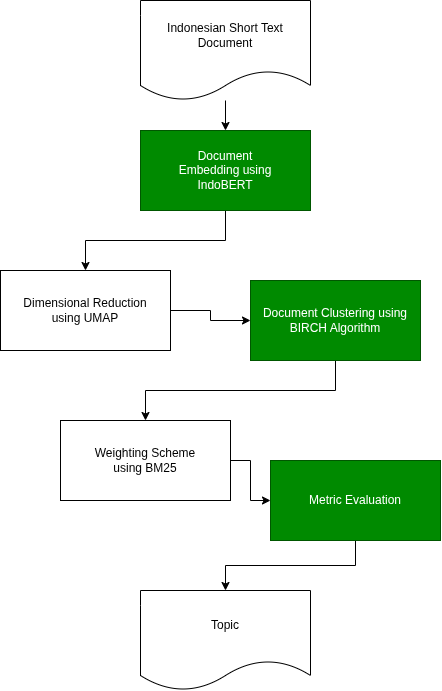
\includegraphics[width=0.45\textwidth]{images/framework-bertopic-modifikasi-indobert-birch-bm25.png}
	\caption{Framework BERTopic dengan modifikasi IndoBERT, BIRCH, dan BM25 \citep{iaes2025indobert}}
	\label{fig:framework-bertopic}
\end{figure}

Berdasarkan Gambar \ref{fig:framework-bertopic}, \textit{framework} BERTopic terdiri dari empat tahap utama. Tahap pertama adalah
\textit{document embedding} yang mengubah dokumen menjadi representasi vektor
numerik menggunakan model bahasa seperti IndoBERTweet yang dikembangkan untuk variasi bahasa Indonesia pada ranah media sosial \citep{koto2021indobertweet}. Tahap kedua adalah
\textit{dimensionality reduction} menggunakan UMAP untuk mereduksi dimensi vektor
hasil \textit{embedding} agar proses klasterisasi lebih efisien \citep{mcinnes2018umap}.
Tahap ketiga adalah \textit{clustering} yang mengelompokkan dokumen berdasarkan
kemiripan semantik, di mana setiap klaster merepresentasikan satu topik dengan
dukungan model yang bersifat modular seperti HDBSCAN, BIRCH, dan K-Means.
Tahap keempat adalah \textit{topic representation} yang mengekstrak kata kunci paling
representatif dari setiap klaster. Secara bawaan BERTopic menggunakan c-TF-IDF,
namun tahap ini dapat dimodifikasi karena bersifat modular \citep{grootendorst2022bertopic}.
Dalam penelitian ini, komponen yang digunakan pada tiap tahap meliputi IndoBERTweet
untuk \textit{embedding}, BIRCH untuk klasterisasi, dan BM25 untuk representasi topik.

% --- BAGIAN 2.3: KERANGKA KONSEPTUAL (OPSIONAL) ---
\subsection{IndoBERTweet}
\label{subsec:indobertweet}

Model IndoBERTweet merupakan model bahasa pra-latih berskala besar pertama yang dirancang khusus untuk memproses data Twitter (X) berbahasa Indonesia.
Model ini dikembangkan melalui pendekatan \textit{domain-adaptive pretraining} dengan fondasi IndoBERT yang semula dilatih pada korpus formal, kemudian diadaptasi ke domain Twitter yang lebih informal.
Dalam proses adaptasi tersebut, peneliti melakukan penyesuaian kosakata domain-spesifik dan melaporkan 14.584 kosakata baru (46\% dari total kosakata) yang tidak tercakup pada IndoBERT umum \citep{koto2021indobertweet}.

\begingroup
\pagestyle{fancy}
\renewcommand{\arraystretch}{1}
\begin{table}[H]
	\centering
	\caption{Perbandingan Kinerja Model pada Tujuh Tugas}\label{tab:kinerja-indobertweet}
	\setlength{\tabcolsep}{4pt}
	\scriptsize
	\begin{tabular}{>{\arraybackslash}p{3.8cm}ccccccc>{\centering\arraybackslash}p{1.5cm}}
		\toprule
		\multirow{2}{*}{{\textbf{Model}}}                                          & \multicolumn{2}{c}{\textbf{Sentiment}} & \textbf{Emotion} & \multicolumn{2}{c}{\textbf{Hate Speech}} & \multicolumn{2}{c}{\textbf{NER}} & \multirow{2}{*}{\parbox{2cm}{\textbf{Average}}}                                                       \\
		\cmidrule(lr){2-3}\cmidrule(lr){4-4}\cmidrule(lr){5-6}\cmidrule(lr){7-8}
		                                                                           & \textbf{IndoLEM}                       & \textbf{SmSA}    & \textbf{EmoT}                            & \textbf{HS1}                     & \textbf{HS2}                                    & \textbf{Formal} & \textbf{Informal} &               \\
		\midrule
		mBERT                                                                      & 76.6                                   & 84.7             & 67.5                                     & 85.1                             & 75.1                                            & 85.2            & 83.2              & 79.6          \\
		malayBERT                                                                  & 82.0                                   & 84.1             & 74.2                                     & 85.0                             & 81.9                                            & 81.9            & 81.3              & 81.5          \\
		IndoBERT \citep{wilie2020indonlu}                                          & 84.1                                   & 88.7             & 73.3                                     & 86.8                             & 80.4                                            & 86.3            & 84.3              & 83.4          \\
		IndoBERT \citep{Indobert2020}                                              & 84.1                                   & 87.9             & 71.0                                     & 86.4                             & 79.3                                            & 88.0            & 86.9              & 83.4          \\
		IndoBERTweet (1M steps from scratch) \citep{koto2021indobertweet}          & 86.2                                   & 90.4             & 76.0                                     & \textbf{88.8}                    & \textbf{87.5}                                   & \textbf{88.1}   & 85.4              & 86.1          \\
		IndoBERT + Vocabulary adaptation + 200K steps \citep{koto2021indobertweet} & \textbf{86.6}                          & \textbf{92.7}    & \textbf{79.0}                            & 88.4                             & 84.0                                            & 87.7            & \textbf{86.9}     & \textbf{86.5} \\
		\bottomrule
	\end{tabular}
\end{table}
\endgroup


Berdasarkan Tabel \ref{tab:kinerja-indobertweet} yang diadaptasi dari \cite{koto2021indobertweet}, model IndoBERTweet dan variannya subsecara konsisten mencapai performa tinggi pada tujuh tugas NLP berbahasa Indonesia, meliputi \textit{sentiment analysis}, \textit{emotion classification}, \textit{hate speech detection}, dan \textit{named entity recognition}.
Hasil terbaik secara rata-rata ditunjukkan oleh varian IndoBERT dengan adaptasi kosakata dan pelatihan lanjutan 200K langkah (86{,}5), sedangkan IndoBERTweet yang dilatih dari awal juga menunjukkan kinerja kompetitif (86{,}1).
Temuan ini memperkuat asumsi bahwa model berbasis domain media sosial berpotensi lebih sesuai untuk teks pendek, informal, dan bising seperti percakapan grup WhatsApp berbahasa Indonesia, meskipun efektivitas akhirnya tetap perlu divalidasi pada penelitian ini.


\subsection{BIRCH Clustering}
\label{subsec:birch}

BIRCH (\textit{Balanced Iterative Reducing and Clustering using Hierarchies}) merupakan algoritma \textit{clustering}
hierarkis yang dirancang untuk menangani dataset berskala besar secara efisien dengan cara meringkas data ke dalam
struktur \textit{Clustering Feature} (CF) yang disusun dalam CF-Tree di memori, sehingga mengurangi kebutuhan komputasi
dibandingkan pendekatan yang memproses setiap titik data secara individual \citep{10.1145/235968.233324}.
Algoritma ini memiliki keunggulan dalam efisiensi komputasi, penggunaan memori yang rendah, serta ketahanan
terhadap \textit{noise}, namun tetap memiliki keterbatasan, seperti sensitivitas terhadap parameter \textit{threshold},
kesulitan dalam menangani klaster dengan bentuk kompleks, serta kurang optimal pada dataset berdimensi tinggi \citep{10.1023/A:1009783824328}.
Dalam konteks framework BERTopic, keterbatasan terkait dimensi tinggi tersebut dapat diminimalkan melalui
penerapan UMAP sebagai teknik reduksi dimensi sebelum proses klasterisasi dilakukan.

Pada implementasi BIRCH di \textit{scikit-learn}, ringkasan tiap subklaster disimpan
dalam bentuk \textit{Clustering Feature} (CF) sebagaimana didefinisikan pada BIRCH
orisinil dan dipaparkan kembali pada kajian implementasi matematis modern
\citep{10.1145/235968.233324,IJECE25896}:

\begin{equation}
	CF = (N, LS, SS)
\end{equation}

\noindent dengan $N$ jumlah titik data, $LS = \sum_{i=1}^{N} x_i$, dan
$SS = \sum_{i=1}^{N} \lVert x_i \rVert^2$.

Centroid subklaster dihitung sebagai:

\begin{equation}
	\mu = \frac{LS}{N}
\end{equation}

Radius subklaster digunakan sebagai dasar keputusan pemisahan/penggabungan node.
Bentuk komputasional berikut ekuivalen dengan definisi radius BIRCH
\citep{10.1145/235968.233324,IJECE25896}:

\begin{equation}
	R = \sqrt{\frac{SS}{N} - \left\lVert \frac{LS}{N} \right\rVert^2}
\end{equation}

Ketika titik baru $x$ ditambahkan ke subklaster, radius baru dihitung menggunakan
prinsip aditivitas CF, lalu dibandingkan dengan \textit{threshold} ($T$)
\citep{10.1145/235968.233324,IJECE25896}:

\begin{equation}
	R' = \sqrt{\frac{SS + \lVert x \rVert^2}{N+1} - \left\lVert \frac{LS + x}{N+1} \right\rVert^2}, \quad R' \le T
\end{equation}

Parameter \textit{branching factor} ($B$) mengontrol jumlah maksimum anak pada tiap
node CF-Tree, sedangkan $T$ mengontrol kekompakan subklaster.


\subsection{Topic Representation Dengan BM25}
\label{sec:bm25}

% TODO: Revisi menambahkan penjelasan mengenai kenapa kok BM25 ini dipakai pada penelitian ini
    Skema pembobotan BM25 adalah algoritma fungsi peringkat (ranking function) yang banyak digunakan dalam pencarian informasi (information retrieval) dan dapat diadaptasi untuk tahap representasi topik \citep{doi.org/10.1111/coin.12248,DBLP:journals/corr/abs-2007-05186}. 
	c-TF-IDF kesulitan menangkap hubungan semantik secara utuh dan cenderung menghasilkan topik yang kurang koheren ketika distribusi frekuensi kata sangat timpang atau tidak merata \citep{iaes2025indobert}. Oleh karena itu, sejumlah
penelitian menerapkan BM25 pada tahap \textit{topic representation}, baik sebagai
pengganti penuh maupun sebagai modifikasi dari skema c-TF-IDF.

Pada penelitian \citep{iaes2025indobert}, c-TF-IDF bawaan BERTopic digantikan
sepenuhnya dengan BM25 pada level klaster, dengan skor kata dirumuskan sebagai:
\begin{equation}
	w_{t,c_k} = \sum_{d \in C_k} IDF(t) \cdot
	\frac{f(t,d)(k_1 + 1)}
	{f(t,d) + k_1 \left(1 - b + b \cdot \frac{|d|}{avgdl}\right)},
\end{equation}
dengan fungsi \textit{inverse document frequency} didefinisikan sebagai
$IDF(t) = \log \left( \frac{N - n(t) + 0.5}{n(t) + 0.5} \right)$.
Skor $w_{t,c_k}$ pada persamaan tersebut dihitung dengan menjumlahkan kontribusi
seluruh dokumen $d$ yang menjadi anggota himpunan dokumen pada klaster ke-$k$,
yang dinotasikan sebagai $C_k$. Untuk setiap dokumen tersebut, $f(t,d)$
menyatakan frekuensi kemunculan kata $t$ di dalam dokumen $d$, sementara $|d|$
menyatakan panjang dokumen $d$ yang kemudian dinormalisasi terhadap $avgdl$,
yaitu rata-rata panjang dokumen dalam korpus. Adapun nilai $IDF(t)$ diperoleh
dari $n(t)$, yang menyatakan jumlah dokumen dalam korpus yang memuat kata $t$,
serta $N$ yang menyatakan jumlah total dokumen dalam korpus tersebut. Dua
parameter tambahan, $k_1$ dan $b$, masing-masing berfungsi mengatur tingkat
saturasi frekuensi istilah agar pengaruh kata yang berulang tidak meningkat
secara linear, dan mengatur normalisasi panjang dokumen agar dokumen yang
lebih panjang tidak secara otomatis memperoleh skor yang lebih tinggi.

Dalam konteks studi tersebut, pendekatan ini dilaporkan memberikan representasi
topik yang lebih stabil dibandingkan c-TF-IDF pada korpus teks pendek berbahasa
Indonesia \citep{iaes2025indobert}.

\subsection{Topic Coherence}
\label{subsec:topic-coherence}

\textit{Topic coherence} digunakan untuk mengukur keterkaitan semantik antar kata teratas dalam topik. Dari banyaknya \textit{topic coherence}, penelitian ini menggunakan \textit{Normalized Pointwise Mutual Information} (NPMI) karena memberikan korelasi tertinggi dengan penilaian manusia dalam konteks context vectors \citep{2685324}:

\begin{equation}
    \text{NPMI}(w_i, w_j) = 
    \frac{
        \log \dfrac{P(w_i, w_j)}{P(w_i) \cdot P(w_j)}
    }{
        -\log P(w_i, w_j)
    }
    \label{eq:npmi-standalone}
\end{equation}

\noindent dengan $P(w_i,w_j)$ sebagai probabilitas ko-okurensi, serta $P(w_i)$ dan $P(w_j)$ sebagai probabilitas
marjinal kemunculan kata. Nilai dari NPMI berkisar antara [-1, 1], dengan nilai 1 menunjukkan keterkaitan semantik yang sempurna, 0 menunjukkan tidak ada keterkaitan, dan nilai negatif menunjukkan keterkaitan yang berlawanan \citep{11271424}.

\subsection{Topic Diversity}
\label{subsec:topic-diversity}

\textit{Topic diversity} didefinisikan dengan keberagaman topik sebagai persentase kata unik dalam 25 kata teratas dari semua topik. Keberagaman mendekati 0 menunjukan bahwa topik yang berlebihan dan keberagaman mendekati 1 menunjukkan topik yang beragam \citep{dieng2020topic}. Nilainya dihitung
melalui rumus berikut:

\begin{equation}
	TD = \frac{|\text{unique words in top } N \text{ words of all topics}|}{N \times K}
\end{equation}

\subsection{Embedding Density}
\label{subsec:embedding-density}

\textit{Embedding Density} adalah metrik evaluasi yang mengukur tingkat kekompakan (\textit{compactness}) representasi embedding dokumen di dalam suatu klaster atau topik \citep{2009-00672}. Metrik ini dihitung menggunakan fungsi kernel dengan bobot sebagai berikut:

\begin{equation}
\rho_k(z) =
\frac{
\sum_{i=1}^{N_k} K\!\left(\dfrac{z - \mathbf{e}_i^{(k)}}{h}\right) w_{k,i}
}{
\sum_{i=1}^{N_k} K\!\left(\dfrac{z - \mathbf{e}_i^{(k)}}{h}\right)
}
\label{eq:embedding-density}
\end{equation}

\noindent dengan $z$ adalah titik embedding evaluasi, yang dalam
penelitian ini ditetapkan sebagai centroid embedding topik $k$
($z = \bar{\mathbf{e}}^{(k)}$); $\mathbf{e}_i^{(k)}$ adalah vektor
embedding dokumen ke-$i$ dalam topik $k$; $N_k$ adalah jumlah dokumen
dalam topik $k$; $K(\cdot)$ adalah fungsi kernel Gaussian; $h$ adalah
parameter \textit{bandwidth}; dan $w_{k,i}$ adalah bobot representativitas
dokumen ke-$i$ terhadap topik $k$, yang dihitung berdasarkan
\textit{cosine similarity} antara embedding dokumen dan centroid
embedding topik tersebut. Semakin tinggi nilai kepadatan yang diperoleh, semakin kohesif dan bermakna topik yang dihasilkan \citep{2009-00672}.

\subsection{Intra-topic Similarity}
\label{subsec:intra-topic-similarity}

Intra-topic similarity merupakan metrik evaluasi yang mengukur kemiripan 
semantik antar dokumen di dalam satu topik, diadaptasi dari konsep 
\textit{intra-list similarity} (ILS) sebagai rata-rata kemiripan berpasangan 
seluruh item dalam sebuah daftar \citep{10.1007/s11257-022-09351-w}. \cite{zhao2018inter} menekankan bahwa struktur intra-topik berbasis 
\textit{word embeddings} mampu menangkap aspek tematik yang lebih halus dan 
bermakna. Dalam konteks evaluasi model topik, intra-topic similarity untuk 
topik $k$ dengan $N_k$ dokumen dirumuskan sebagai berikut:
\begin{equation}
    \text{ITS}(k) = \frac{1}{N_k(N_k - 1)} 
        \sum_{\substack{i,j=1 \\ i \neq j}}^{N_k}
        \cos\!\left(\mathbf{e}_i^{(k)},\, \mathbf{e}_j^{(k)}\right)
    \label{eq:intra-topic-similarity}
\end{equation}

\noindent di mana $\mathbf{e}_i^{(k)}$ dan $\mathbf{e}_j^{(k)}$ adalah 
embedding dokumen ke-$i$ dan ke-$j$ dalam topik $k$. Nilai akhir diperoleh 
dengan merata-ratakan $\text{ITS}(k)$ di seluruh $K$ topik; semakin tinggi 
nilainya, semakin kohesif topik yang dihasilkan.

% Gunakan diagram jika tersedia (lihat contoh di bawah):
% \begin{figure}[h]
% \centering
% \includegraphics{images/conceptual-framework.png}
% \caption{Kerangka Konseptual Penelitian}
% \label{fig:framework}
% \end{figure}

% ====================================================================
% CATATAN PENGISIAN BAB TINJAUAN PUSTAKA:
%
% 1. PENELITIAN TERDAHULU:
%    - Minimal 10 referensi (sesuai juknis)
%    - Urutkan secara kronologis atau tematik
%    - Highlight gap/celah yang akan Anda isi
%    - Cite dengan benar (gunakan Mendeley/Zotero)
%
% 2. LANDASAN TEORI:
%    - Jelaskan teori relevan (2-4 teori utama)
%    - Gunakan subsection untuk mengorganisir
%    - Berikan konteks dan aplikasi praktis dari teori
%    - Jangan hanya copy-paste, jelaskan dengan kata-kata Anda
%
% 3. KERANGKA KONSEPTUAL:
%    - Hubungkan teori dengan penelitian Anda
%    - Jelaskan variabel independen, dependen, kontrol (jika ada)
%    - Bisa dalam bentuk deskripsi atau diagram
%    - Ini adalah "jembatan" antara teori dan metodologi
%
% 4. SITASI:
%    - Gunakan format APA (sesuai juknis)
%    - Minimal 50% referensi dari 10 tahun terakhir
%    - Tambah file references.bib untuk bibliography
% ====================================================================


% BAB 3: METODOLOGI PENELITIAN
% ====================================================================
% BAB 3: METODOLOGI PENELITIAN
% ====================================================================
% File ini berisi metodologi penelitian yang mencakup:
% - Lokasi dan waktu penelitian
% - Populasi dan sampel
% - Data penelitian (jenis dan sumber)
% - Prosedur penelitian
% - Metode analisis
%
% EDIT konten sesuai dengan metodologi penelitian Anda.
% ====================================================================

\chapter{METODOLOGI PENELITIAN}

% --- BAGIAN 3.1: LOKASI DAN WAKTU PENELITIAN ---
\section{Jenis Penelitian}
\label{sec:method-type}

Penelitian ini termasuk kategori kuantitatif eksperimental dengan pendekatan Research and Development (R\&D).
Aspek R\&D terletak pada pengembangan sistem analisis topik percakapan WhatsApp berbasis web,
sedangkan aspek eksperimental kuantitatif digunakan untuk memvalidasi performa pipeline BERTopic dengan modifikasi IndoBERTweet sebagai model embedding dan BIRCH sebagai model clustering yang diimplementasikan dalam sistem.

% --- BAGIAN 3.2: POPULASI DAN SAMPEL ---
\section{Objek Penelitian}
\label{sec:method-object}

Objek penelitian fokus pada data percakapan grup WhatsApp yang berisi
interaksi antar pengguna dalam bahasa Indonesia. Data ini dipilih karena
mewakili karakteristik percakapan yang umumnya berupa teks pendek, tidak
terstruktur, mengandung \textit{noise}, serta fenomena \textit{code-mixing}.
Karakteristik tersebut menjadikan data percakapan grup WhatsApp relevan untuk
menguji kemampuan pipeline BERTopic yang dimodifikasi dalam menghasilkan topik
yang koheren dan stabil.

\section{Waktu Penelitian}
\label{sec:time}

Waktu penelitian dilakukan pada bulan April 2026 hingga Juni 2026, dengan tahapan-tahapan yang telah direncanakan secara sistematis untuk memastikan kelancaran proses penelitian.

\section{Tahapan Penelitian}
\label{sec:stages}

Tahapan penelitian yang dilakukan dalam penelitian ini secara keseluruhan
digambarkan pada \textbf{Gambar \ref{fig:tahapan-penelitian}}:

\begin{figure}[H]
	\centering
	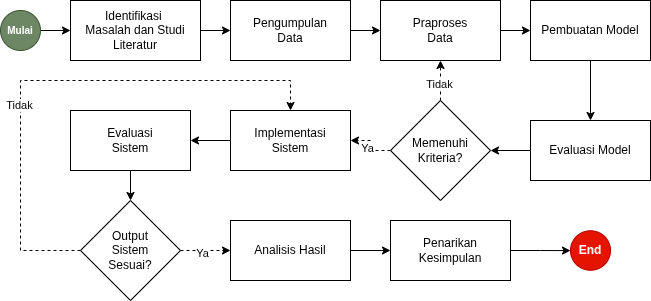
\includegraphics[width=0.85\textwidth]{images/alur_penelitian.png}
	\caption{Tahapan Penelitian}
	\label{fig:tahapan-penelitian}
\end{figure}

\subsection{Identifikasi Masalah dan Studi Literatur}
\label{subsec:problem-identification}

Tahap pertama dalam penelitian ini adalah identifikasi masalah dan studi
literatur. Peneliti melakukan eksplorasi awal terhadap fenomena percakapan grup
WhatsApp untuk memahami tantangan dalam menangkap topik pembicaraan secara
menyeluruh, mencakup dinamika percakapan, karakteristik teks, serta kebutuhan
pengguna dalam mengelola informasi yang besar dan tidak terstruktur.

Studi literatur kemudian dilakukan untuk membangun landasan teori dan memahami
perkembangan terkini di bidang \textit{topic modeling} berbahasa Indonesia melalui
kajian jurnal ilmiah, prosiding konferensi, dan dokumentasi teknis terkait BERTopic,
IndoBERTweet, BIRCH \textit{clustering}, BM25, serta metrik evaluasi pemodelan topik.
Hasil gabungan tahap ini digunakan untuk mengidentifikasi \textit{research gap},
merumuskan masalah penelitian secara spesifik, dan menentukan metode serta
arsitektur sistem yang akan dikembangkan.

\subsection{Pengumpulan Data}
\label{subsec:data-collection}

Tahap pengumpulan data dilakukan dengan mengekspor riwayat percakapan dari grup
WhatsApp menggunakan fitur \textit{export chat} yang tersedia secara bawaan pada
aplikasi WhatsApp. Data yang diekspor berupa file teks (\textit{.txt}) atau format \textit{.zip} yang memuat
informasi tanggal, waktu, nama pengirim, dan isi pesan. Data percakapan yang
dikumpulkan hanya bersumber dari satu grup WhatsApp, dengan rentang waktu maksimal
satu tahun data terbaru untuk memastikan relevansi topik dan menjaga fokus analisis
pada dinamika percakapan yang aktual.

\subsection{Praproses Data}
\label{subsec:data-preprocessing}

Tahap pra-pemrosesan data dibagi menjadi dua tahap, yaitu sebelum
\textit{embedding} model dan sebelum representasi topik.

\noindent \textbf{Tahap 1: Pra-\textit{Embedding} Model}

\noindent Tahap ini bertujuan membersihkan dan mempersiapkan data mentah agar siap diolah
oleh model \textit{embedding} dengan tetap mempertahankan makna semantik. Prosesnya meliputi:
\begin{enumerate}[nosep]
	\item Pemfilteran pesan sistem, yaitu menghapus notifikasi bawaan
	      WhatsApp seperti pesan bergabung, keluar grup, perubahan keamanan,
	      serta pesan media yang tidak disertakan.
	\item Konversi teks menjadi huruf kecil (\textit{lower-case}).
	\item Normalisasi \textit{mention} dan URL, dengan mengganti
	      nama pengguna menjadi \textit{@USER} dan URL menjadi \textit{HTTP}.
	\item Transliterasi emotikon.
	\item Normalisasi kata slang dan pemanjangan kata.
\end{enumerate}

\noindent \textbf{Tahap 2: Pra-Representasi Topik}

\noindent Tahap ini dilakukan sebelum pembentukan representasi topik, yaitu dengan
konfigurasi \textit{vectorizer} menggunakan \textit{stopword} dari kamus manual
dan \textit{library} Sastrawi.

\subsection{Pembuatan Model}
\label{subsec:create-model}

Tahap pemodelan topik merupakan tahap inti dari penelitian ini, di mana data
yang telah melalui pra-pemrosesan dianalisis menggunakan \textit{framework} BERTopic
yang telah dimodifikasi. Penentuan parameter pada tiap komponen dilakukan dengan
dua skenario, yaitu mengacu pada \textit{baseline} dari penelitian terdahulu dan
eksperimen penalaan parameter untuk memperoleh kinerja terbaik berdasarkan metrik
evaluasi. Alur pembuatan model ini terdiri dari empat komponen utama:

\begin{figure}[H]
	\centering
	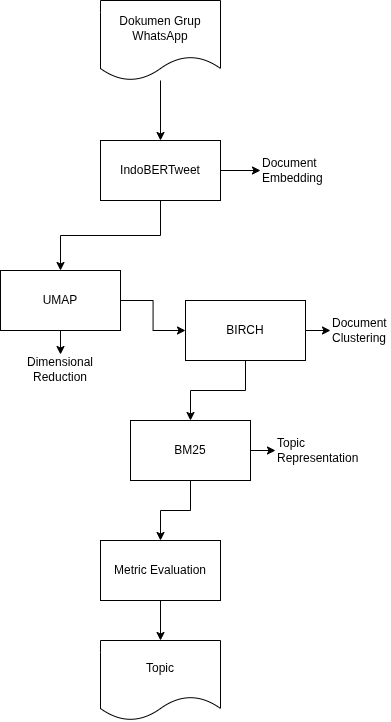
\includegraphics[width=0.5\textwidth]{images/framework-BERTopic-modifikasi.png}
	\caption{Rancangan framework BERTopic yang dimodifikasi pada tahap pembuatan model}\label{fig:framework-bertopic-modifikasi}
\end{figure}

\begin{enumerate}[nosep]
	\item \textbf{\textit{Document Embedding} menggunakan IndoBERTweet} \\
	      Setiap dokumen (pesan) diubah menjadi representasi vektor numerik
	      berdimensi tinggi menggunakan model IndoBERTweet yang telah diadaptasi
	      untuk teks media sosial berbahasa Indonesia. Representasi \textit{embedding} ini
	      mampu menangkap makna semantik dan konteks kata secara lebih akurat
	      dibandingkan model \textit{multilingual} \citep{koto2021indobertweet}.

	\item \textbf{\textit{Dimensionality Reduction} menggunakan UMAP} \\
	      Vektor \textit{embedding} berdimensi tinggi direduksi menggunakan
	      \textit{Uniform Manifold Approximation and Projection} (UMAP) untuk
	      mengurangi kompleksitas komputasi sambil mempertahankan struktur lokal
	      dan global data dalam ruang berdimensi rendah. Parameter UMAP yang
	      digunakan meliputi \textit{n\_neighbors}, \textit{n\_components},
	      \textit{min\_dist}, dan \textit{metric}.

	\item \textbf{\textit{Clustering} menggunakan BIRCH} \\
	      Dokumen yang telah direduksi dimensinya dikelompokkan menggunakan
	      algoritma BIRCH (\textit{Balanced Iterative Reducing and Clustering
		      using Hierarchies}) sebagai pengganti HDBSCAN standar. BIRCH dipilih
	      karena kemampuannya dalam mengalokasikan seluruh dokumen ke dalam
	      klaster tanpa menghasilkan \textit{outlier} dalam jumlah besar, serta
	      efisiensi komputasi dan penggunaan memori yang lebih baik. Parameter
	      BIRCH yang digunakan meliputi \textit{threshold},
	      \textit{branching\_factor}, dan \textit{n\_clusters}.

	\item \textbf{\textit{Topic Representation} menggunakan BM25} \\
	      Setiap klaster yang terbentuk direpresentasikan menggunakan skema
	      pembobotan BM25 sebagai pengganti c-TF-IDF bawaan BERTopic. BM25
	      menerapkan saturasi frekuensi istilah dan normalisasi panjang dokumen,
	      sehingga menghasilkan kata kunci representatif yang lebih relevan dan
	      stabil secara semantik untuk setiap topik. Parameter BM25 yang digunakan
	      meliputi \textit{k1} dan \textit{b}.
\end{enumerate}

\subsection{Evaluasi Model}
\label{subsec:model-evaluation}

Tahap evaluasi model bertujuan untuk mengukur kualitas topik yang dihasilkan
oleh model BERTopic secara kuantitatif. Evaluasi dilakukan menggunakan empat
metrik utama, yaitu:
\begin{enumerate}[nosep]
	\item \textit{Topic Coherence} (NPMI) untuk mengukur sejauh mana
	      kata-kata teratas dalam setiap topik memiliki hubungan semantik satu
	      sama lain. Nilai yang lebih tinggi menunjukkan topik yang lebih koheren.
	\item \textit{Topic Diversity} (TD) untuk mengukur keunikan kata-kata
	      teratas antar topik. Nilai mendekati 1 menunjukkan tidak ada tumpang
	      tindih kata antar topik.
	\item \textit{Embedding Density} untuk mengukur tingkat kekompakan
	      dokumen dalam tiap klaster pada ruang \textit{embedding}. Nilai yang
	      lebih tinggi menunjukkan klaster yang semakin padat.
	\item \textit{Intra-topic Similarity} untuk mengukur rata-rata
	      kesamaan semantik antar dokumen dalam satu topik. Nilai yang lebih
	      tinggi menunjukkan homogenitas topik yang lebih baik.
\end{enumerate}

\subsection{Implementasi Sistem}
\label{subsec:system-implementation}

Tahap pengembangan sistem bertujuan untuk mengimplementasikan seluruh alur
pemodelan topik ke dalam sebuah aplikasi berbasis web yang dapat digunakan
secara praktis oleh pengguna. Sistem ini memungkinkan pengguna untuk mengunggah
data ekspor percakapan grup WhatsApp, melakukan analisis topik secara otomatis,
serta menampilkan hasil pemodelan topik dalam bentuk visualisasi yang intuitif
dan informatif. Implementasi dilakukan dengan arsitektur \textit{client-server},
dengan Vue.js sebagai \textit{client} (antarmuka pengguna) dan FastAPI sebagai
\textit{server} (layanan API pemrosesan analisis topik). Pengembangan sistem
dilakukan menggunakan pendekatan terstruktur dengan memperhatikan aspek
fungsionalitas, kemudahan penggunaan (\textit{usability}), dan efisiensi
pemrosesan.

\subsection{Evaluasi Sistem}
\label{subsec:system-evaluation}

Tahap evaluasi sistem dilakukan untuk mengukur kinerja dan efektivitas aplikasi	yang telah dikembangkan. Evaluasi dilakukan dengan menggunakan metode black-box testing, di mana fokusnya adalah pada input dan output sistem tanpa memperhatikan proses internalnya. Pengujian dilakukan dengan menggunakan dataset percakapan grup WhatsApp yang berbeda dari dataset yang digunakan untuk pelatihan model, untuk memastikan bahwa sistem dapat bekerja secara umum dan tidak hanya pada data tertentu. Hasil evaluasi ini akan memberikan gambaran tentang seberapa baik sistem dapat mengidentifikasi dan merepresentasikan topik dalam percakapan grup WhatsApp secara otomatis, serta memberikan umpan balik untuk perbaikan lebih lanjut jika diperlukan.

\subsection{Analisis Hasil}
\label{subsec:result}

Tahap analisis hasil dilakukan terhadap seluruh keluaran dari pemodelan topik
dan evaluasi model. Analisis dilakukan dengan membandingkan performa model
berdasarkan metrik evaluasi yang telah ditentukan, serta menginterpretasikan
topik-topik yang dihasilkan.

\subsection{Penarikan Kesimpulan}

Berdasarkan hasil analisis, dilakukan penarikan kesimpulan yang menjawab
rumusan masalah penelitian serta penyusunan saran untuk pengembangan penelitian
di masa mendatang.

% ====================================================================
% CATATAN PENGISIAN BAB METODOLOGI:
%
% 1. LOKASI & WAKTU:
%    - Spesifik dan jelas (bukan abstrak)
%    - Jelaskan alasan pemilihan lokasi
%    - Sertakan durasi penelitian
%
% 2. POPULASI & SAMPEL:
%    - Definisikan populasi dengan jelas
%    - Jelaskan kriteria inklusi/eksklusi
%    - Tunjukkan perhitungan ukuran sampel
%    - Jelaskan metode sampling
%
% 3. DATA:
%    - Sebutkan jenis data (primer/sekunder, kualitatif/kuantitatif)
%    - Jelaskan sumber data spesifik
%    - Descripsikan instrumen pengumpulan data
%    - Sertakan validitas/reliabilitas instrumen
%
% 4. PROSEDUR:
%    - Urut kronologis dan logis
%    - Detail namun tidak berbelit-belit
%    - Jelaskan setiap tahap dengan jelas
%
% 5. ANALISIS:
%    - Jelaskan teknik analisis deskriptif
%    - Jelaskan uji statistik (jika ada) dengan detail
%    - Sertakan asumsi-asumsi uji
%    - Sebutkan software yang digunakan
% ====================================================================


% BAB 4: HASIL DAN PEMBAHASAN
% ====================================================================
% BAB 4: HASIL DAN PEMBAHASAN
% ====================================================================
% File ini berisi hasil penelitian dan pembahasan yang mencakup:
% - Hasil penelitian (data terolah dan temuan utama)
% - Pembahasan hasil (interpretasi dan analisis kritis)
%
% EDIT konten sesuai dengan hasil penelitian Anda.
% ====================================================================

\chapter{HASIL DAN PEMBAHASAN}


\section{Pengumpulan Data}
\label{sec:data-collection}

Data penelitian diperoleh dari grup percakapan WhatsApp [nama/deskripsi grup] setelah memperoleh izin dari admin grup sebagaimana dijelaskan pada Lampiran~\ref{subsec}. 
Pengumpulan data dilakukan menggunakan fitur \textit{Export Chat} bawaan aplikasi WhatsApp, yang menghasilkan berkas dalam format \textit{.zip} berisi riwayat percakapan dalam satu berkas \textit{.txt} tanpa media. 
Berkas \textit{.zip} tersebut terlebih dahulu diekstraksi untuk memperoleh file \textit{.txt} yang selanjutnya digunakan sebagai sumber data utama penelitian. 
Data yang diekspor mencakup periode percakapan dari [tanggal awal] hingga [tanggal akhir], dengan total [jumlah] pesan dari [jumlah] partisipan grup.

Sebagai ilustrasi, potongan data mentah hasil ekspor ditampilkan pada Listing~\ref{lst:contoh-data-mentah}. 
Secara umum, setiap baris percakapan mengikuti pola \texttt{DD/MM/YY HH.MM - Pengirim: Pesan}. 
Namun demikian, data mentah juga memuat variasi format lain seperti pesan sistem (misalnya anggota ditambahkan ke grup), placeholder media, tautan, dan penanda pesan yang telah diedit.

\begin{lstlisting}[caption={Contoh potongan data mentah hasil ekspor WhatsApp (nama disamarkan)}, label={lst:contoh-data-mentah}, basicstyle=\ttfamily\small]
02/02/26 20.46 - User-1: Woi Katakan pada dunia hsr back
02/02/26 20.47 - User-1: <Media tidak disertakan>
27/09/25 10.35 - User-3: sheesh
03/02/26 11.24 - User-4: https://link
28/09/25 09.48 - User-5: gara gara dapet evernight jadi pengen hyacine <Pesan ini diedit>
24/04/26 05.12 - User-7 sudah ditambahkan
\end{lstlisting}

Berkas \textit{.txt} selanjutnya diproses melalui tahap \textit{parsing} menggunakan \textit{regular expression} untuk mengekstrak tiga atribut utama, yaitu \textit{Timestamp}, \textit{Pengirim}, dan \textit{Pesan}. 
Pada tahap ini, nilai \textit{timestamp} dinormalisasi ke format ISO 8601 (\texttt{YYYY-MM-DDTHH:MM}) untuk memudahkan pengurutan kronologis, filtering temporal, dan analisis berbasis waktu.

Sebagai ilustrasi, hasil \textit{parsing} dari potongan data mentah pada Listing~\ref{lst:contoh-data-mentah} disajikan pada Tabel~\ref{tab:contoh-hasil-parsing}.

\begingroup
\pagestyle{fancy}
\renewcommand{\arraystretch}{1}
\begin{table}[H]
\centering
\caption{Contoh Hasil Parsing Data WhatsApp ke Format CSV}
\label{tab:contoh-hasil-parsing}
\scriptsize
\begin{tabular}{p{12cm}}
\toprule
\textbf{Pesan} \\
\midrule
Woi Katakan pada dunia hsr back \\
sheesh \\
https://link \\
gara gara dapet evernight jadi pengen hyacine \\
\bottomrule
\end{tabular}
\end{table}
\endgroup

\section{Praproses Data}
\label{sec:preprocessing}
\noindent Uraikan langkah pra-pemrosesan yang dilakukan sesuai metodologi:
\begin{enumerate}[nosep]
    \item Pemfilteran pesan sistem dan pesan media
    \item Normalisasi (lower-case, mention → @USER, URL → HTTP)
    \item Transliteration emotikon dan normalisasi slang
    \item Tokenisasi dan stopword removal (Sastrawi + manual)
\end{enumerate}
Berikan contoh before/after satu atau dua pesan untuk ilustrasi.

\section{Pembuatan Model}
\label{sec:descriptive-results}
\noindent Sajikan statistik deskriptif utama setelah pra-pemrosesan: mean, median, standar deviasi panjang pesan, frekuensi kata teratas, dan distribusi topik awal jika relevan.

\subsection{Embedding dan Reduksi Dimensi}
\label{subsec:embedding-umap}
\noindent Jelaskan penggunaan IndoBERTweet untuk pembuatan embedding, parameter penting yang dipilih, dan hasil reduksi dimensi menggunakan UMAP. Sertakan visualisasi (scatter plot UMAP) dan interpretasi singkat.

\subsection{Clustering dan Representasi Topik}
\label{subsec:clustering-topics}
\noindent Paparkan penggunaan BIRCH untuk clustering dan BM25 untuk representasi topik. Untuk setiap topik utama, tampilkan:
\begin{itemize}[nosep]
    \item Kata kunci representatif (top-n)
    \item Jumlah dokumen per klaster
    \item Contoh pesan yang termasuk dalam topik
\end{itemize}

\subsection{Evaluasi Kuantitatif Model}
\label{subsec:model-evaluation}
\noindent Tampilkan hasil metrik evaluasi yang digunakan: topic coherence, topic diversity, embedding density, dan intra-topic similarity. Sajikan hasil dalam tabel per skenario parameter (baseline vs modifikasi) dan beri interpretasi singkat.

\subsection{Perbandingan Eksperimen (Baseline vs Modifikasi)}
\label{subsec:experiments-comparison}
\noindent Bandingkan kinerja skenario berbeda (mis. HDBSCAN vs BIRCH, c-TF-IDF vs BM25, model embedding berbeda). Sertakan tabel ringkasan dan highlight perbedaan signifikan.

\subsection{Uji Asumsi dan Analisis Inferensial}
\label{subsec:inferential-results}
\noindent Jika relevan, laporkan uji normalitas, uji homogenitas, dan hasil pengujian hipotesis. Jelaskan metode statistik yang digunakan dan implikasinya terhadap interpretasi hasil.

\subsection{Implementasi Sistem dan Evaluasi Fungsional}
\label{subsec:system-evaluation}
\noindent Laporkan hasil pengujian aplikasi berbasis web: keandalan upload, waktu proses end-to-end, pengalaman pengguna (jika ada pengujian usability), serta contoh tampilan hasil.

\subsection{Analisis Hasil}
\label{subsec:result-analysis}
\noindent Analisis sintesis hasil kuantitatif dan kualitatif: apakah topik yang dihasilkan bermakna, stabil, dan sesuai konteks grup WhatsApp. Kaitkan dengan tujuan penelitian.

% --- BAGIAN 4.2: PEMBAHASAN ---
\section{Pembahasan}
\label{sec:discussion}

\subsection{Interpretasi Temuan Utama}
\label{subsec:interpretation}
\noindent Paparkan penjelasan mendalam mengenai temuan utama, mengapa hasil tersebut muncul, dan bagaimana temuan ini menjawab rumusan masalah. Hubungkan temuan dengan teori dan tinjauan pustaka di Bab 2.

\subsection{Analisis Kualitatif Topik}
\label{subsec:qualitative-topic-analysis}
\noindent Bahas beberapa topik penting secara kualitatif: konteks sosialnya, contoh kutipan pesan, dan relevansi bagi pengguna.

\subsection{Implikasi Praktis dan Rekomendasi Implementasi}
\label{subsec:practical-implications}
\noindent Jelaskan implikasi untuk pengembangan sistem dan pengguna akhir, termasuk rekomendasi konfigurasi model, antarmuka, dan fitur tambahan.

\subsection{Keterbatasan Penelitian}
\label{subsec:limitations}
\noindent Sebutkan keterbatasan data, metode, dan eksperimen (mis. satu grup WhatsApp, potensi bias, keterbatasan anotasi) serta dampaknya pada generalisasi hasil.

\subsection{Saran dan Pekerjaan Lanjutan}
\label{subsec:future-work}
\noindent Rekomendasi teknis dan riset lanjutan: perluasan dataset, eksperimen model embedding lain, perbaikan pipeline pra-pemrosesan, atau pengujian usability yang lebih formal.

\subsection{Ringkasan Hasil Utama}
\label{subsec:summary-results}
\noindent Ringkas temuan paling penting dalam 3--5 poin yang langsung menjawab rumusan masalah.

% ====================================================================
% CATATAN: Isi tiap subsection diisi dengan hasil eksperimen dan pembahasan spesifik Anda.
% Gunakan tabel dan gambar sesuai kebutuhan, dan rujuk ke Bab 3 untuk metodologi yang relevan.
% ====================================================================

% ====================================================================
% CATATAN PENGISIAN BAB HASIL & PEMBAHASAN:
%
% 1. HASIL PENELITIAN:
%    - Presentasikan data secara objektif (tidak interpretasi)
%    - Gunakan tabel dan grafik untuk clarity
%    - Jelaskan setiap temuan utama
%    - Gunakan statistik deskriptif dengan tepat
%
% 2. PEMBAHASAN - SANGAT PENTING:
%    - JANGAN hanya repeat hasil, JELASKAN MENGAPA
%    - Hubungkan dengan teori dan literature dari Bab 2
%    - Analisis kritis: apakah sejalan/berbeda dengan penelitian terdahulu?
%    - Jelaskan implikasi praktis
%    - Sertakan keterbatasan penelitian
%    - Inilah bagian "value-add" dari skripsi Anda
%
% 3. FORMAT:
%    - Gunakan subsection untuk mengorganisir topik
%    - Gunakan referensi ke tabel/gambar: "seperti terlihat pada Tabel \ref{tab:label}"
%    - Sertakan kutipan dari literature: \citet{Author2020}
%
% 4. ELEMEN KRITIS:
%    - Analisis mendalam (bukan permukaan)
%    - Kritisisme terhadap hasil: apa artinya? kenapa terjadi?
%    - Perbandingan dengan studi sebelumnya
%    - Keterbatasan yang jujur dan transparan
% ====================================================================


% BAB 5: KESIMPULAN DAN SARAN
% ====================================================================
% BAB 5: KESIMPULAN DAN SARAN
% ====================================================================
% File ini berisi kesimpulan dan saran penelitian yang mencakup:
% - Kesimpulan (menjawab rumusan masalah secara komprehensif)
% - Saran (rekomendasi akademik dan praktis)
% ====================================================================

\chapter{KESIMPULAN DAN SARAN}

% --- BAGIAN 5.1: KESIMPULAN ---
\section{Kesimpulan}
\label{sec:conclusion}

Berdasarkan seluruh rangkaian tahapan penelitian, perancangan sistem, implementasi, serta pengujian dan evaluasi kuantitatif yang telah dilaksanakan pada data percakapan grup WhatsApp, diperoleh beberapa kesimpulan utama yang menjawab rumusan masalah penelitian sebagai berikut:

\begin{enumerate}
    \item \textbf{Penerapan Modified BERTopic pada Percakapan WhatsApp:} \\
    Penelitian ini berhasil merancang dan menerapkan modifikasi arsitektur \textit{framework} BERTopic yang disesuaikan secara spesifik untuk menangani karakteristik wacana percakapan grup WhatsApp berbahasa Indonesia. Integrasi alur \textit{Single-Path Preprocessing} berhasil mereduksi derau (\textit{noise}) dan membersihkan 91.868 pesan mentah menjadi 56.089 dokumen berkualitas tinggi. Pada tahap pemodelan, pemanfaatan model bahasa \textit{embedding} IndoBERTweet (vektor 768 dimensi), reduksi dimensi UMAP (5 komponen dengan metrik kosinus), algoritma pengklasteran hierarkis BIRCH (\textit{BirchWithOutliers} dengan \textit{threshold} 0,25 dan batas persentil pencilan 95,0), representasi BM25 ($k_1 = 1,2; b = 0,5$) yang diperkaya kamus \textit{STOPWORDS} 9 kategori, serta reduksi topik otomatis dengan mekanisme pengaman (\textit{safety guard}) terbukti mampu mengekstraksi topik percakapan secara terstruktur dan adaptif.

    \item \textbf{Kualitas dan Performa Model Usulan Dibandingkan Baseline:} \\
    Hasil pengujian kurva pembelajaran (\textit{learning curve}) pada proporsi 20\% hingga 100\% data menunjukkan bahwa model usulan (\textit{proposed}) secara konsisten mengungguli model \textit{baseline} BERTopic standar pada seluruh aspek evaluasi kuantitatif:
    \begin{enumerate}[label=\alph*.]
        \item \textit{Pengurangan Outlier Rate}: Penggunaan algoritma BIRCH berhasil menekan persentase dokumen pencilan secara drastis dari 42,42\% pada \textit{baseline} menjadi hanya \textbf{8,79\%} pada model usulan (pada 100\% data), sehingga mempertahankan lebih dari 91\% volume percakapan ke dalam klaster topik yang valid.
        \item \textit{Peningkatan Koherensi Topik (C-NPMI)}: Model usulan menghasilkan nilai koherensi semantik kata kunci yang meningkat signifikan dari 0,0662 (\textit{baseline}) menjadi \textbf{0,1567}, membuktikan bahwa representasi IndoBERTweet dan BM25 mampu menghasilkan kata kunci topik yang padu dan relevan secara makna percakapan informal.
        \item \textit{Stabilitas Keberagaman Topik (Topic Diversity)}: Nilai \textit{Topic Diversity} pada model usulan terjaga sangat tinggi pada skor \textbf{0,9559} (rentang 0,9335--0,9919), yang mengonfirmasi bahwa kata kunci antartopik tidak mengalami tumpang-tindih (\textit{redundancy}) berkat penyaringan \textit{stopwords} 9 kategori.
        \item \textit{Kepadatan Vektor dan Kemiripan Internal Klaster}: Model usulan mencapai \textit{Embedding Density} sebesar \textbf{0,6666} (vs 0,5611 pada \textit{baseline}) dan \textit{Intra-topic Similarity} sebesar \textbf{0,6716} (vs 0,5211 pada \textit{baseline}), menegaskan bahwa klaster topik yang terbentuk memiliki batas kerapatan yang tegas serta tingkat homogenitas semantik yang erat.
    \end{enumerate}

    \item \textbf{Perancangan dan Implementasi Sistem Web Terintegrasi:} \\
    Penelitian ini berhasil merancang dan mengimplementasikan sistem analisis percakapan grup WhatsApp berbasis web (\textit{ChatAnalisis}) dengan arsitektur \textit{client-server} yang memisahkan antarmuka pengguna (\textit{frontend} Vue.js 3, TypeScript, TailwindCSS, Pinia) dan layanan pemrosesan komputasi (\textit{backend} FastAPI terakselerasi GPU/CUDA). Sistem mengintegrasikan fitur privasi data melalui \textit{client-side salted SHA-256 anonymization}, pemrosesan latar belakang asinkron (\textit{BackgroundTasks}), pemantauan progres \textit{real-time} berbasis \textit{Server-Sent Events} (SSE), penelusuran konteks pesan historis (\textit{message context traceability}), proteksi keamanan \textit{path traversal}, dan pembersihan berkas disk otomatis. Pengujian fungsional sistem menggunakan metode \textit{Black-Box Testing} terhadap 34 skenario kasus uji menunjukkan bahwa seluruh fitur pada modul antarmuka dan API \textit{backend} beroperasi 100\% valid sesuai dengan spesifikasi kebutuhan.
\end{enumerate}

Secara keseluruhan, integrasi IndoBERTweet, BIRCH \textit{clustering}, dan skema representasi BM25 pada \textit{framework} BERTopic yang diwujudkan dalam aplikasi web interaktif telah terbukti secara empiris dan aplikatif mampu menjadi solusi komprehensif dalam mengatasi tantangan \textit{information overload} serta ekstraksi wawasan tematik pada percakapan grup WhatsApp berskala besar.

% --- BAGIAN 5.2: SARAN ---
\section{Saran}
\label{sec:recommendations}

Berdasarkan hasil temuan penelitian, evaluasi sistem, serta keterbatasan yang dihadapi selama pelaksanaan penelitian, berikut adalah beberapa saran yang dapat diajukan untuk pengembangan akademik selanjutnya dan implementasi praktis:

\subsection{Saran untuk Penelitian Selanjutnya}
\label{subsec:future-research}

\begin{enumerate}
    \item \textbf{Eksplorasi Model Bahasa dan Arsitektur Embedding Mutakhir:} \\
    Penelitian selanjutnya dapat mengeksplorasi perbandingan performa menggunakan model bahasa generasi terbaru, seperti model berbasis \textit{Large Language Models} (LLM) berbahasa Indonesia atau model representasi kalimat dwibahasa mutakhir, guna menguji peningkatan pemahaman semantik pada percakapan dengan tingkat \textit{code-mixing} yang lebih kompleks.

    \item \textbf{Pengembangan Pemodelan Topik Dinamis (Dynamic Topic Modeling):} \\
    Penelitian dapat diperluas dengan menambahkan dimensi waktu (\textit{temporal dynamics}) untuk mengamati pergeseran dan evolusi topik percakapan dari waktu ke waktu (\textit{topic drift}), sehingga tren pembicaraan komunitas dapat dipetakan secara kronologis per periode tertentu.

    \item \textbf{Integrasi Analisis Wacana Lanjutan:} \\
    Pengembangan dapat mengombinasikan pemodelan topik dengan analisis sentimen, analisis emosi, atau analisis jejaring sosial (\textit{Social Network Analysis}) untuk memahami polaritas opini anggota kelompok dan pola interaksi sosial di dalam setiap tema pembicaraan.

    \item \textbf{Pengujian pada Domain dan Format Perangkat Beragam:} \\
    Disarankan untuk menguji generalisabilitas model pada domain percakapan grup yang berbeda (seperti grup koordinasi kerja, komunitas akademik, atau layanan publik) serta memperluas format data masukan dari sistem operasi lain (misalnya berkas ekspor chat dari perangkat iOS).
\end{enumerate}

\subsection{Saran untuk Praktisi dan Pengembangan Terapan}
\label{subsec:practical-recommendations}

\begin{enumerate}
    \item \textbf{Dukungan Multi-Platform Aplikasi Pesan Instan:} \\
    Pengembang aplikasi dapat menambahkan fitur penguraian (\textit{parser}) untuk platform pesan instan lainnya, seperti Telegram, Discord, atau Slack, sehingga platform web analisis ini dapat digunakan secara universal oleh berbagai komunitas digital.

    \item \textbf{Peningkatan Skalabilitas dan Manajemen Antrean Server:} \\
    Untuk implementasi pada lingkungan produksi berskala besar dengan banyak pengguna bersamaan (\textit{concurrent users}), disarankan untuk mengintegrasikan sistem antrean tugas terdistribusi (seperti Celery dan Redis) serta orkestrasi kontainer (Docker/Kubernetes).

    \item \textbf{Fitur Ekspor Laporan dan Notifikasi Berkala:} \\
    Disarankan untuk menambahkan fitur ekspor laporan hasil analisis topik ke dalam format PDF/Excel interaktif serta modul ringkasan berkala yang dapat dikirimkan secara otomatis kepada administrator grup.
\end{enumerate}


% ====================================================================
% BAGIAN 3: BACK MATTER (BAGIAN AKHIR)
% ====================================================================

% Daftar Pustaka (Bibliography)
% ====================================================================
% DAFTAR PUSTAKA (BIBLIOGRAPHY)
% ====================================================================
% File ini berisi daftar referensi/pustaka yang digunakan dalam penelitian.
% Format: APA Style (sesuai Juknis UNEJ)
%
% PETUNJUK PENGGUNAAN:
% 1. Gunakan file references.bib untuk menyimpan semua referensi
% 2. Uncomment baris di bawah untuk mengaktifkan daftar pustaka
% 3. Compile dengan: pdflatex → bibtex → pdflatex → pdflatex
% ====================================================================

\setlength{\bibsep}{0pt} % Mengurangi spasi antar referensi (opsional)
\renewcommand{\bibname}{%
\begin{center}
    {\normalfont\bfseries\fontsize{14pt}{16pt}\selectfont DAFTAR PUSTAKA}
\end{center}
\vspace*{-1cm}
}
\addcontentsline{toc}{chapter}{DAFTAR PUSTAKA}

% --- MENGGUNAKAN BIBTEX (AKTIF) ---
% Gunakan file daftar_pustaka.bib untuk menyimpan semua referensi
\bibliographystyle{apalike}
\bibliography{daftar_pustaka}

% ====================================================================
% PANDUAN PENGUMPULAN REFERENSI:
%
% 1. MINIMAL REFERENSI:
%    - Juknis: minimal 50% dari 10 tahun terakhir
%    - Umumnya: 20-50 referensi untuk skripsi
%
% 2. JENIS SUMBER YANG BAIK:
%    - Academic journals (50-70%)
%    - Books (10-20%)
%    - Conference proceedings (10-20%)
%    - Internet sources (5-15%, hanya yang kredibel)
%    - Grey literature (reports, theses) - minimal 5%
%
% 3. FORMAT MENGGUNAKAN BIBTEX:
%    
%    a) Buat file references.bib:
%       @article{Author2020,
%         title={Title of Paper},
%         author={Author, A. and Others, B.},
%         journal={Journal Name},
%         volume={30},
%         pages={100-115},
%         year={2020},
%         doi={10.xxxx/xxxxx}
%       }
%
%    b) Cite dalam dokumen: \citet{Author2020} atau \citep{Author2020}
%
% 4. TOOLS UNTUK MANAJEMEN REFERENSI:
%    - Mendeley (mendeley.com) - generate .bib file
%    - Zotero (zotero.org) - open source
%    - EndNote - commercial
%    - RefWorks - web-based
%
% 5. GENERATOR BIB FORMAT:
%    - Google Scholar: export ke BibTeX
%    - Semantic Scholar: export BibTeX
%    - CrossRef: provide DOI, convert ke BibTeX
%
% 6. TIPS PENTING:
%    - Gunakan DOI jika tersedia
%    - Pastikan spelling penulis dan tahun AKURAT
%    - Urutan publikasi: Chronological atau Alphabetical
%    - Dalam disiplin ilmu tertentu, format mungkin berbeda
%      (tanyakan pembimbing tentang format yang diharapkan)
% ====================================================================


% Lampiran (Appendices)
% ====================================================================
% LAMPIRAN (APPENDICES)
% ====================================================================
% File ini berisi lampiran penelitian.
% Lampiran dapat mencakup:
% - Data mentah
% - Kode sumber (untuk research komputasi)
% - Tabel detail/besar
% - Instrumen penelitian (kuesioner, interview guide)
% - Dokumen pendukung lainnya
%
% EDIT konten sesuai dengan lampiran penelitian Anda.
% ====================================================================

\appendix
\frontmatterchapter{LAMPIRAN}
\noindent\textbf{Lampiran - Alur Implementasi Sistem}

\begin{figure}[H]
\centering
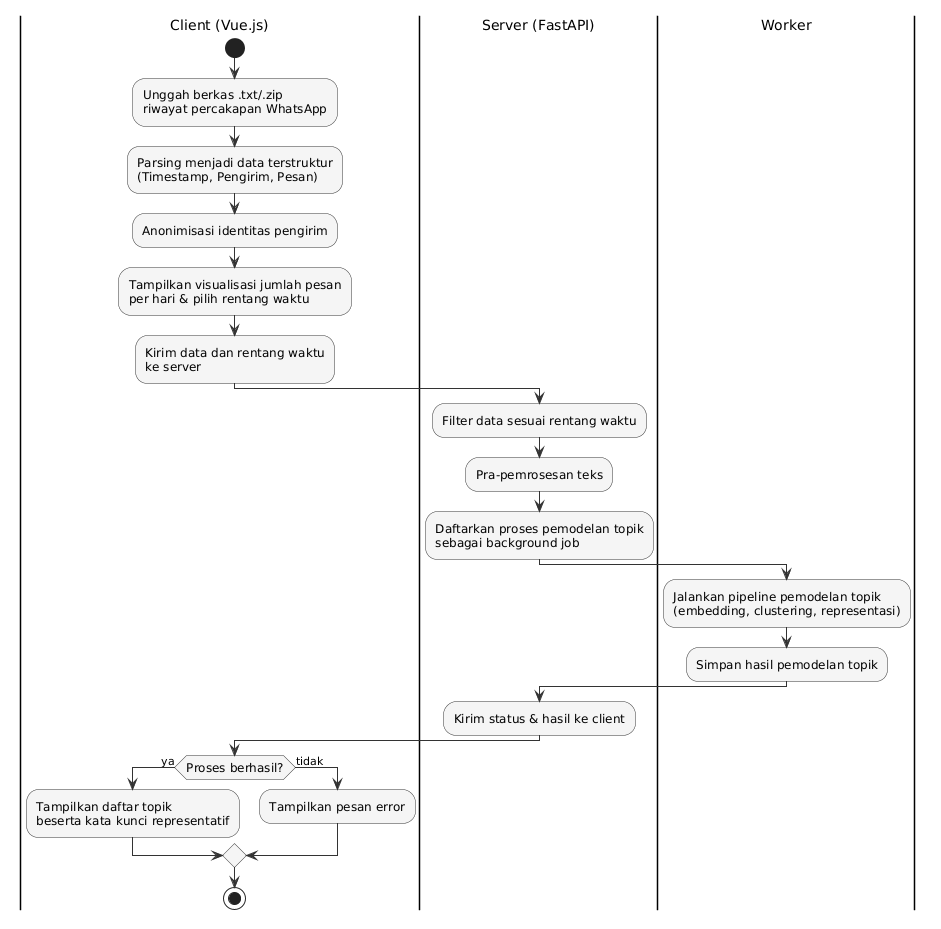
\includegraphics[width=0.9\textwidth]{images/bab-3-alur-implementasi-sistem.png}
\caption{Alur Implementasi Sistem}
\label{fig:bab-3-alur-implementasi-sistem}
\end{figure}

\newpage
\noindent\textbf{Lampiran - Alur Teknis Implementasi Sistem Web}

\begin{figure}[H]
\centering
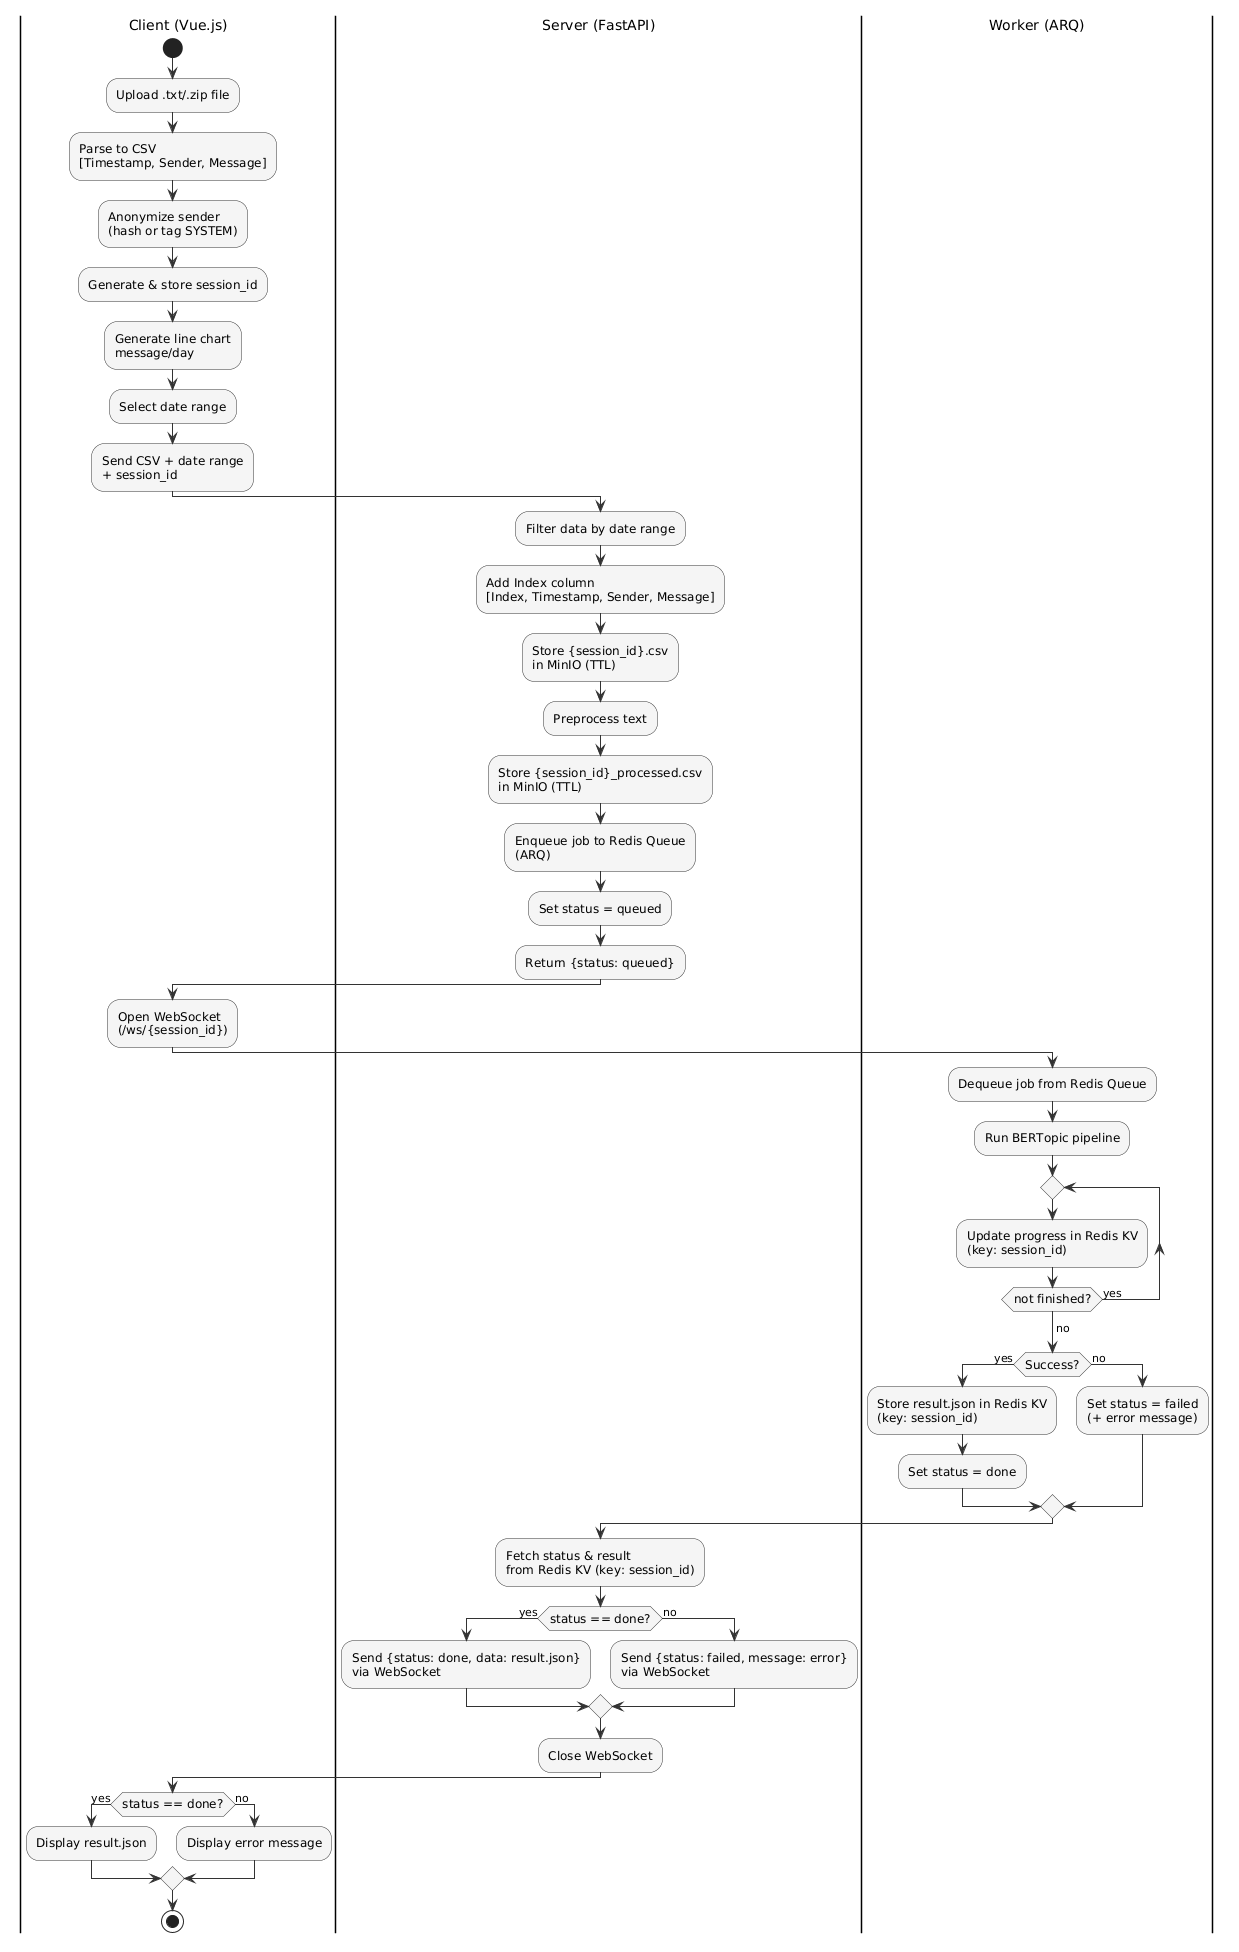
\includegraphics[width=0.9\textwidth]{images/bab-4-alur-teknis-implementasi-sistem.png}
\caption{Alur Teknis Implementasi Sistem}
\label{fig:bab-4-alur-teknis-implementasi-sistem}
\end{figure}


% ====================================================================
% CATATAN PENGISIAN LAMPIRAN:
%
% 1. JENIS LAMPIRAN YANG BIASA DISERTAKAN:
%    - Data mentah (raw data)
%    - Instrumen (kuesioner, interview guide, observation sheet)
%    - Output analisis (tabel detail, grafik dari software)
%    - Kode sumber (untuk komputasi/programming research)
%    - Dokumen administratif (surat izin, ICF, ethical clearance)
%    - Tabel/grafik pendukung yang terlalu besar untuk main text
%
% 2. ORGANISASI:
%    - Gunakan Lampiran A, B, C, dst. untuk kategorisasi
%    - Setiap lampiran harus direferensikan dalam main text
%    - Tambahkan deskripsi untuk clarity
%
% 3. FORMAT:
%    - Lampiran harus jelas dan mudah dibaca
%    - Gunakan numbering, labeling yang konsisten
%    - Sertakan captions dan figure/table references
%
% 4. UKURAN:
%    - Jangan membuat lampiran terlalu besar
%    - Untuk data besar, gunakan external file dan referensikan
%    - Dokumentasi external files dengan jelas
%
% 5. KEAMANAN DATA:
%    - Jangan masukkan data pribadi yang sensitif (nama, nomor identitas)
%    - Anonimisasi data jika diperlukan
%    - Pertimbangkan privasi responden
% ====================================================================


% ====================================================================
% END DOCUMENT
% ====================================================================

\end{document}

% ====================================================================
% DOKUMENTASI & PANDUAN PENGGUNAAN
% ====================================================================
%
% STRUKTUR FOLDER:
% .
% ├── main.tex                    ← File ini (entry point)
% ├── metadata.tex                ← Edit di sini: judul, nama, pembimbing
% ├── config/
% │   ├── packages.tex            ← Semua \usepackage
% │   ├── hyperref-config.tex     ← PDF metadata & hyperlink settings
% │   ├── formatting.tex          ← Format chapter/section/subsection
% │   ├── page-style.tex          ← Header/footer & page numbering
% │   └── custom-commands.tex     ← Custom LaTeX commands & environments
% ├── frontmatter/
% │   ├── 00-cover.tex            ← Halaman sampul
% │   ├── 01-dedication.tex       ← Persembahan
% │   ├── 02-motto.tex            ← Motto
% │   ├── 03-originality.tex      ← Pernyataan orisinalitas
% │   ├── 04-approval.tex         ← Halaman persetujuan & pengesahan
% │   ├── 05-abstract-id.tex      ← Abstrak Indonesia
% │   ├── 06-abstract-en.tex      ← Abstract English
% │   ├── 07-summary.tex          ← Ringkasan
% │   ├── 08-preface.tex          ← Prakata
% │   └── 09-toc.tex              ← Daftar Isi & Gambar & Tabel
% ├── chapters/
% │   ├── 01-introduction.tex     ← BAB 1: Pendahuluan
% │   ├── 02-literature.tex       ← BAB 2: Tinjauan Pustaka
% │   ├── 03-methodology.tex      ← BAB 3: Metodologi Penelitian
% │   ├── 04-results.tex          ← BAB 4: Hasil & Pembahasan
% │   └── 05-conclusion.tex       ← BAB 5: Kesimpulan & Saran
% ├── backmatter/
% │   ├── 01-references.tex       ← Daftar Pustaka
% │   └── 02-appendices.tex       ← Lampiran
% └── README.md                    ← Dokumentasi proyek
%
% ====================================================================
% CARA COMPILE & GENERATE PDF:
% ====================================================================
%
% OPSI 1: Menggunakan pdflatex (Command Line)
% -------------------------------------------
% $ pdflatex main.tex
% $ pdflatex main.tex      # Compile 2x agar TOC, references akurat
% $ pdflatex main.tex      # Compile 3x untuk hasil optimal
%
% Jika ada bibliography:
% $ pdflatex main.tex
% $ bibtex main            # Generate references
% $ pdflatex main.tex
% $ pdflatex main.tex
%
% OPSI 2: Menggunakan latexmk (Otomatis, Rekomendasi)
% ----
% $ latexmk -pdf main.tex  # Otomatis compile berapa kali diperlukan
%
% OPSI 3: Menggunakan VS Code dengan LaTeX Workshop Extension
% ------
% - Install extension: James Yu "LaTeX Workshop"
% - Buka main.tex → Klik 'Build LaTeX project' atau Ctrl+Alt+B
% - PDF akan generate otomatis di folder output/
%
% ====================================================================
% WORKFLOW EDITING FILE:
% ====================================================================
%
% UNTUK MENGUBAH METADATA (Nama, Judul, Pembimbing, dll):
% → Edit file: metadata.tex
%    Semua perubahan akan otomatis ter-update di seluruh dokumen
%
% UNTUK MENGEDIT ISI BAB SPESIFIK:
% → Edit file: chapters/[nomor]-[nama].tex
%    Misalnya untuk Bab 2, edit: chapters/02-literature.tex
%
% UNTUK MENAMBAH CUSTOM COMMAND:
% → Edit file: config/custom-commands.tex
%    Contoh: command untuk format tabel, quote, signature block, dll.
%
% UNTUK MENGUBAH GLOBAL STYLING:
% → Edit file yang relevan di folder config/
%    - Warna link: config/hyperref-config.tex
%    - Font/margin: config/packages.tex
%    - Format heading: config/formatting.tex
%
% ====================================================================
% TIPS & BEST PRACTICES:
% ====================================================================
%
% 1. JANGAN EDIT main.tex
%    Gunakan main.tex hanya untuk structure. Semua content ada di
%    file-file terpisah di folder chapters/, frontmatter/, dll.
%
% 2. GUNAKAN LABEL & REFERENCE
%    Contoh: \label{sec:intro} di section, kemudian \ref{sec:intro}
%    Ini membuat cross-reference otomatis dan robust.
%
% 3. COMPILE SECARA BERKALA
%    Compile saat membuat perubahan besar untuk cek syntax error awal.
%
% 4. GUNAKAN CITATIONS
%    \citet{Author2020} vs \citep{Author2020}
%    Perlu file references.bib untuk bibliography.
%
% 5. COMMENT OUT BAGIAN
%    Gunakan % untuk comment line, atau \iffalse ... \fi untuk block
%    Berguna saat testing atau saat belum siap publish section tertentu.
%
% ====================================================================
% TROUBLESHOOTING:
% ====================================================================
%
% [ERROR] Undefined control sequence
% → Pastikan semua \usepackage sudah diimport di config/packages.tex
%
% [ERROR] File not found
% → Cek path ke file di \input{...} sudah benar relatif ke main.tex
%
% [ERROR] TOC tidak update
% → Compile 2-3 kali, LaTeX perlu multiple pass untuk TOC
%
% [WARNING] Overfull hbox
% → Bisa diabaikan jika minor, atau ubah text/spacing jika serius
%
% ====================================================================
% RESOURCES & DOKUMENTASI:
% ====================================================================
%
% - LaTeX Documentation: https://www.latex-project.org/help/documentation/
% - Comprehensive TeX Archive (CTAN): https://ctan.org/
% - Overleaf Documentation: https://www.overleaf.com/learn
% - Juknis UNEJ: Lihat README.md di repository ini
% - Untuk help LaTeX: tanya di community seperti TeX StackExchange
%
% ====================================================================
